\chapter{Integration Engineering}
\label{sec:fdsp-coord-integ-sysengr}

The \dword{dune} \dword{fd} consists of \dwords{spmod} and
\dwords{dpmod}, housed inside cryostats, which in turn are housed
inside the \dword{lbnf} \dword{fscf}.  This nested structure is
mirrored with detector integration in a similar layered manner.  This
chapter explains the method of integration for the \dwords{detmodule}.
The integration of the modules is carried out by the
\dword{jpo}/\dword{tc} engineering team.

Integration engineering for \dword{dune} focuses on configuring the
mechanical and electrical systems of each \dword{detmodule} and managing
the interfaces within them. This includes verifying that subassemblies
and their interfaces are built conforming to the approved design,
e.g., \dword{apa} or \dword{pds}. The second major focus
is assuring that the \dwords{detmodule} can be integrated and
installed into their final configuration. And the third major focus is
integrating necessary services provided by \dword{cf} 
with the \dwords{detmodule}.


To this end, the \dword{jpo}/\dword{tc} engineering team maintains
subsystem component documentation in order to manage the detector
configuration. The consortia provide engineering data for their
subsystems to \dword{tc}. The \dword{jpo}/\dword{tc} engineering team
works with the \dword{lbnf} project team and \dword{jpo} to integrate
all detector data into the global \dword{lbnf} configuration files.

This process is the same as was used for \dword{protodune}, which proved to be
successful. The process has been enhanced with the addition of engineering
and design staff and development of interface documents as described
in Section~\ref{sec:fdsp-coord-interface}.

\section{Mechanical Integration Models}
\label{sec:fdsp-coord-integ-models}

The \dword{sp} and \dword{dp} \dwords{detmodule} are large and made of many
intricate components. Fortunately, for the most part, the
components are repetitive and not overly complex
geometrically. Thus, \threed mechanical modeling techniques are well suited
to represent the \dwords{detmodule} and manage their configuration.

At the same time, \threed modelling techniques vary in the way items are
represented and in the way the techniques are carried out. Thus, a set
of \twod integration drawings must be generated; these drawings must be
clear and unambiguous across the collaboration. Such \twod drawings are
the basis for the \threed model accuracy, as well as the basis for the engineering
design of all components.

The consortia choose their mechanical modeling software.
Their model files are transferred to \dword{tc}/\dword{jpo} via STEP
files, which the \dword{jpo}/\dword{tc} engineering team integrates
into overall models.  Navisworks software allows for visualization by
the entire collaboration.

\subsection{Static Models}
\label{sec:fdsp-coord-integ-static}

\dword{tc} generates and maintains \threed detector integration models
as well as \twod integration drawings of the detector. These models
are static because they represent all components at their design
dimensions and locations. They do not represent effects of gravity,
tolerances, cold temperature, and installation and assembly
clearances. Such effects are modeled in the envelope and assembly
models, as described in Section~\ref{sec:fdsp-coord-integ-envelope}.


The \threed models are assembled by combining component models from
various consortia, then shared with the consortia. The \twod
integration drawings, which are generated from the \threed models and
disseminated, show the interfaces to the level of detail necessary to
ensure proper fit and function. Any issues that arise are communicated
to the consortia, and a resolution method is determined.

The \dword{jpo}/\dword{tc} engineering team will not change any
consortia component models.  The consortia must resolve any issues
using agreed-upon methods, and provide updated models for
reintegration. Using this process, models are kept synchronized with
integration occurring in only one direction: only the consortia modify
their models, and the \dword{jpo}/\dword{tc} engineering team
integrates and disseminates them.  \dword{jpo}/\dword{tc} will provide
engineering support as needed to keep consortia models
current. \dword{jpo}/\dword{tc} will define points in the design
process where current models are combined and defined as the official
current integration model.

The level of detail in a model is managed actively. When models are
combined and incorporated into global models of facilities, too much
detail leads to very large file sizes.  The \dword{jpo}/\dword{tc}
engineering team must ensure the appropriate level of detail at each
stage of model integration.


Several examples from the \dword{spmod} are presented
here. Figure~\ref{fig:dune-sp_overall} shows the overall model of the
\dword{spmod} with one wall of the cryostat removed to make the
interior components visible. The detector has 25 rows, all of which
follow the same construction. At the ends of rows 1 and 25,
\dwords{ewfc} are installed to close the detection volume.  As mentioned
earlier, this model does not include all the details of the detector
components. The components are simplified to keep the overall model
complexity to a manageable level.
\begin{dunefigure}[Overall model of the SP module]{fig:dune-sp_overall}
  {Overall model of the \dword{spmod} showing three of the 25 rows,
    simplified cryostat, \dword{dss} and temporary cryostat opening.}
  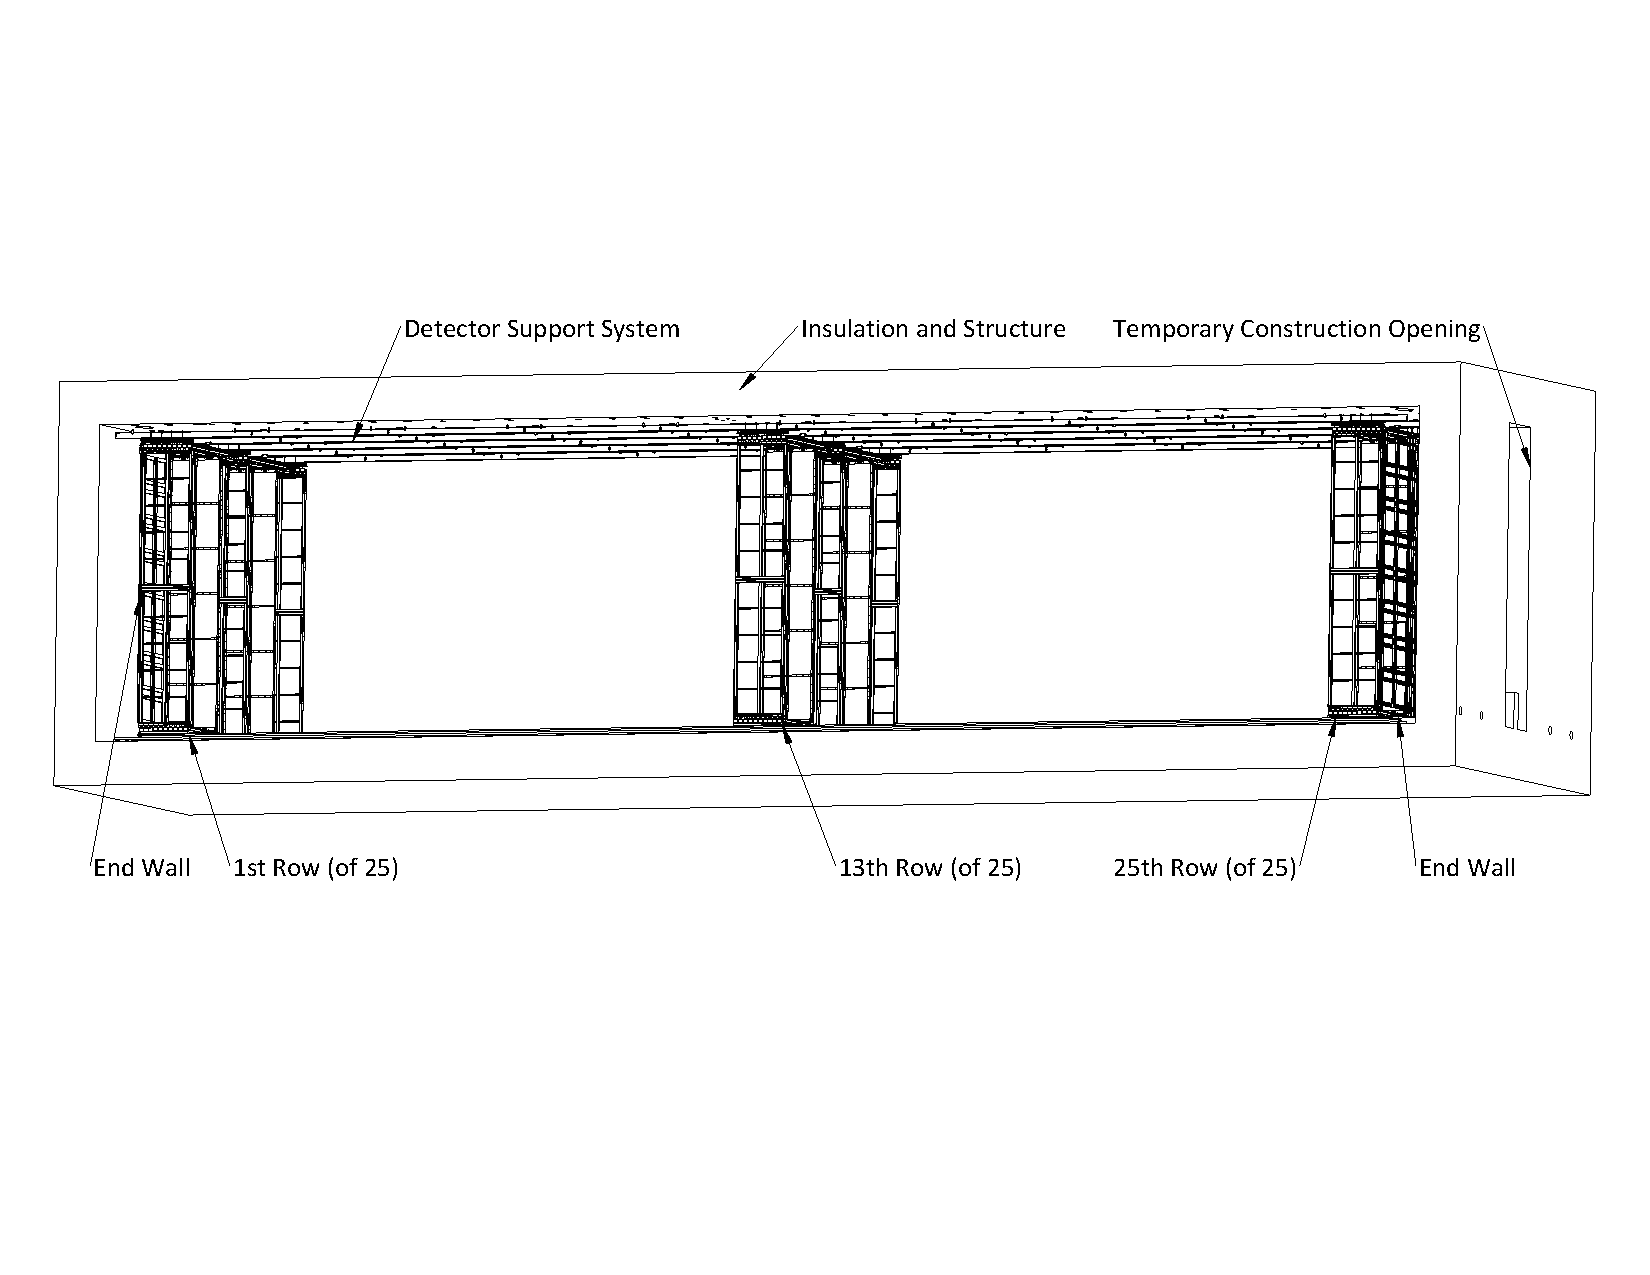
\includegraphics[width=0.85\textwidth]{Overall_model_SP}
\end{dunefigure} 


Figure~\ref{fig:dune-sp_row} shows the model of one row of the
detector module. Each row is constructed from six \dwords{apa}, four
\dwords{cpa} and eight \dwords{fc} and \dwords{gp}. A total of 25 rows
comprise one \dword{spmod}.
\begin{dunefigure}[Model of one row of the SP module]{fig:dune-sp_row}
  {Model of one row of \dword{spmod} showing overall arrangement and dimensions.}
  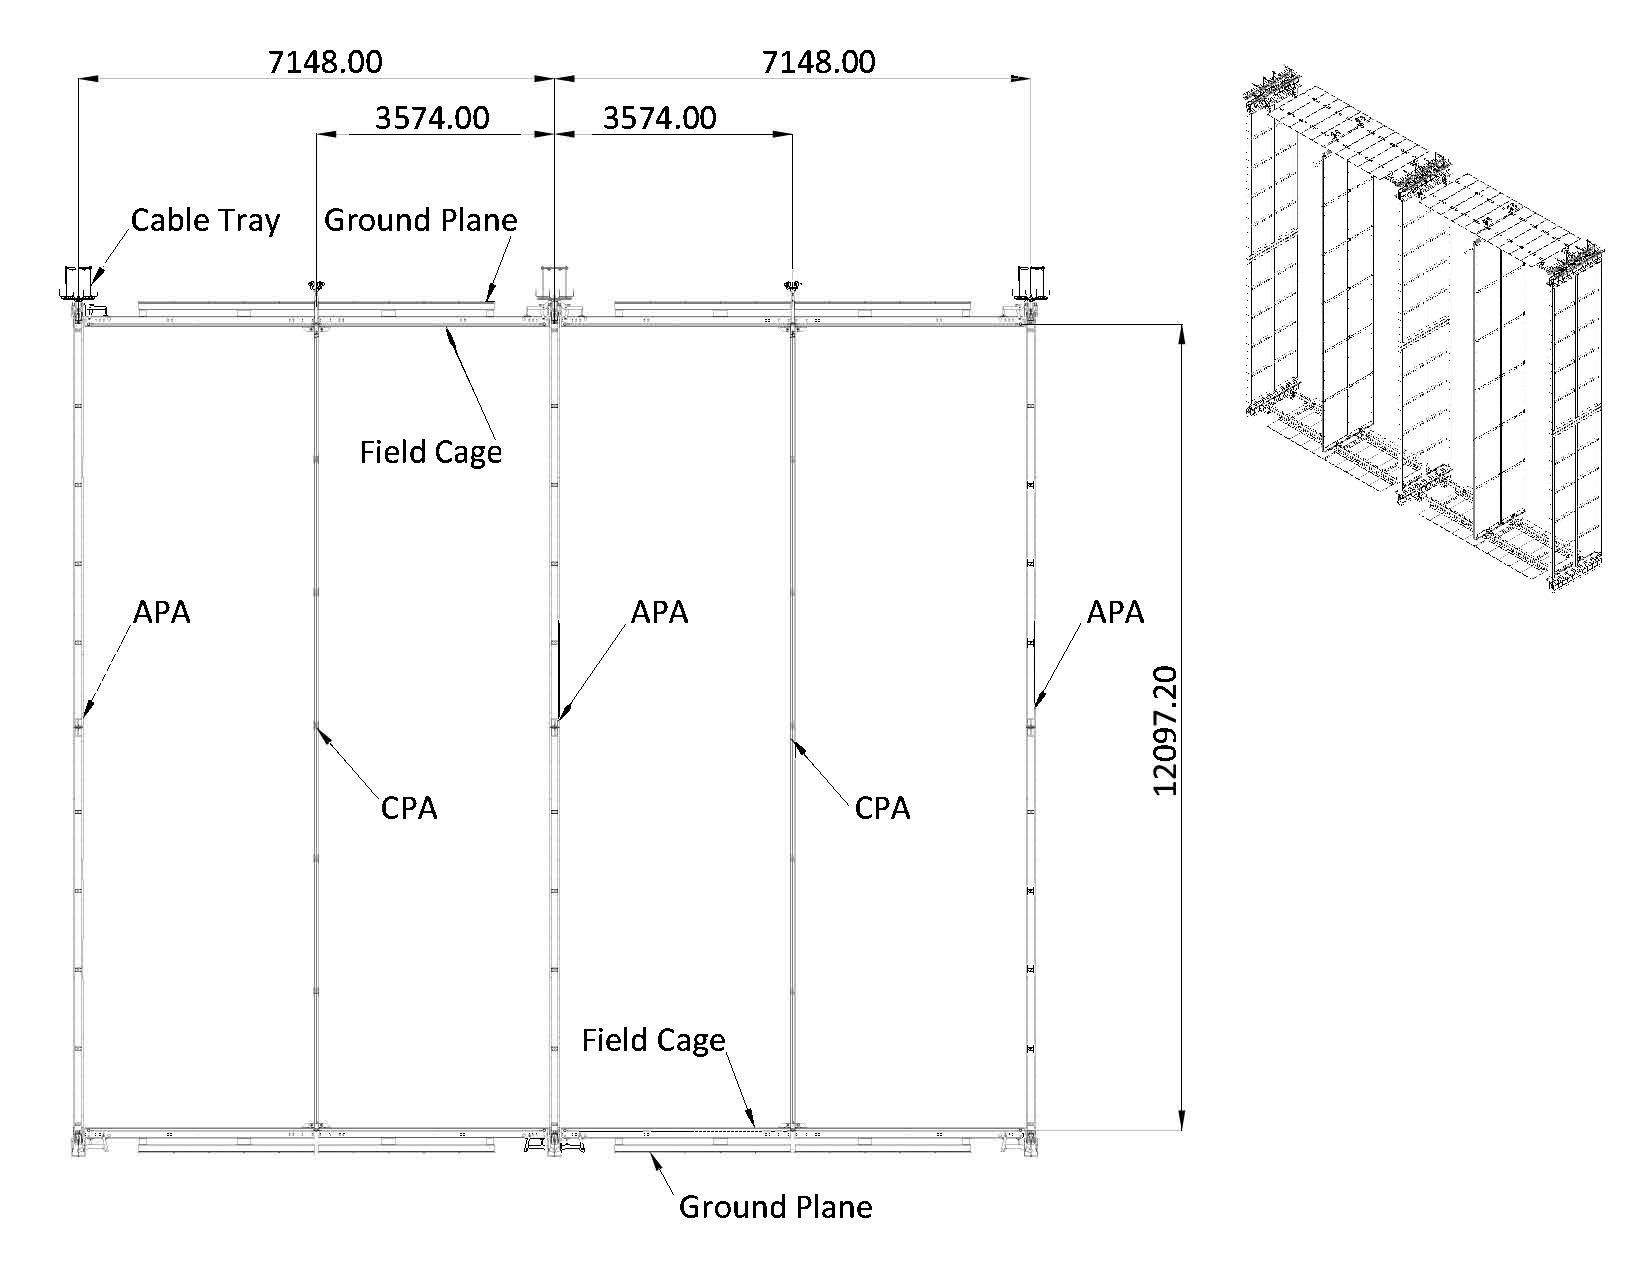
\includegraphics[width=0.85\textwidth]{Model_one_row_SP.pdf}
\end{dunefigure}


Figure~\ref{fig:dune-sp_transverse} shows a cross section of the
\dword{spmod} in the transverse direction and the overall dimensions.
Figure~\ref{fig:dune-sp_long} shows a cross section of the
\dword{spmod} in the longitudinal direction and the overall
dimensions. In both figures, the cryostat structure and insulation are
shown as cross-hatched areas.
\begin{dunefigure}[Section view of the SP module in the
    transverse direction]{fig:dune-sp_transverse}
  {Section view of the \dword{spmod} in the transverse
    direction.}
  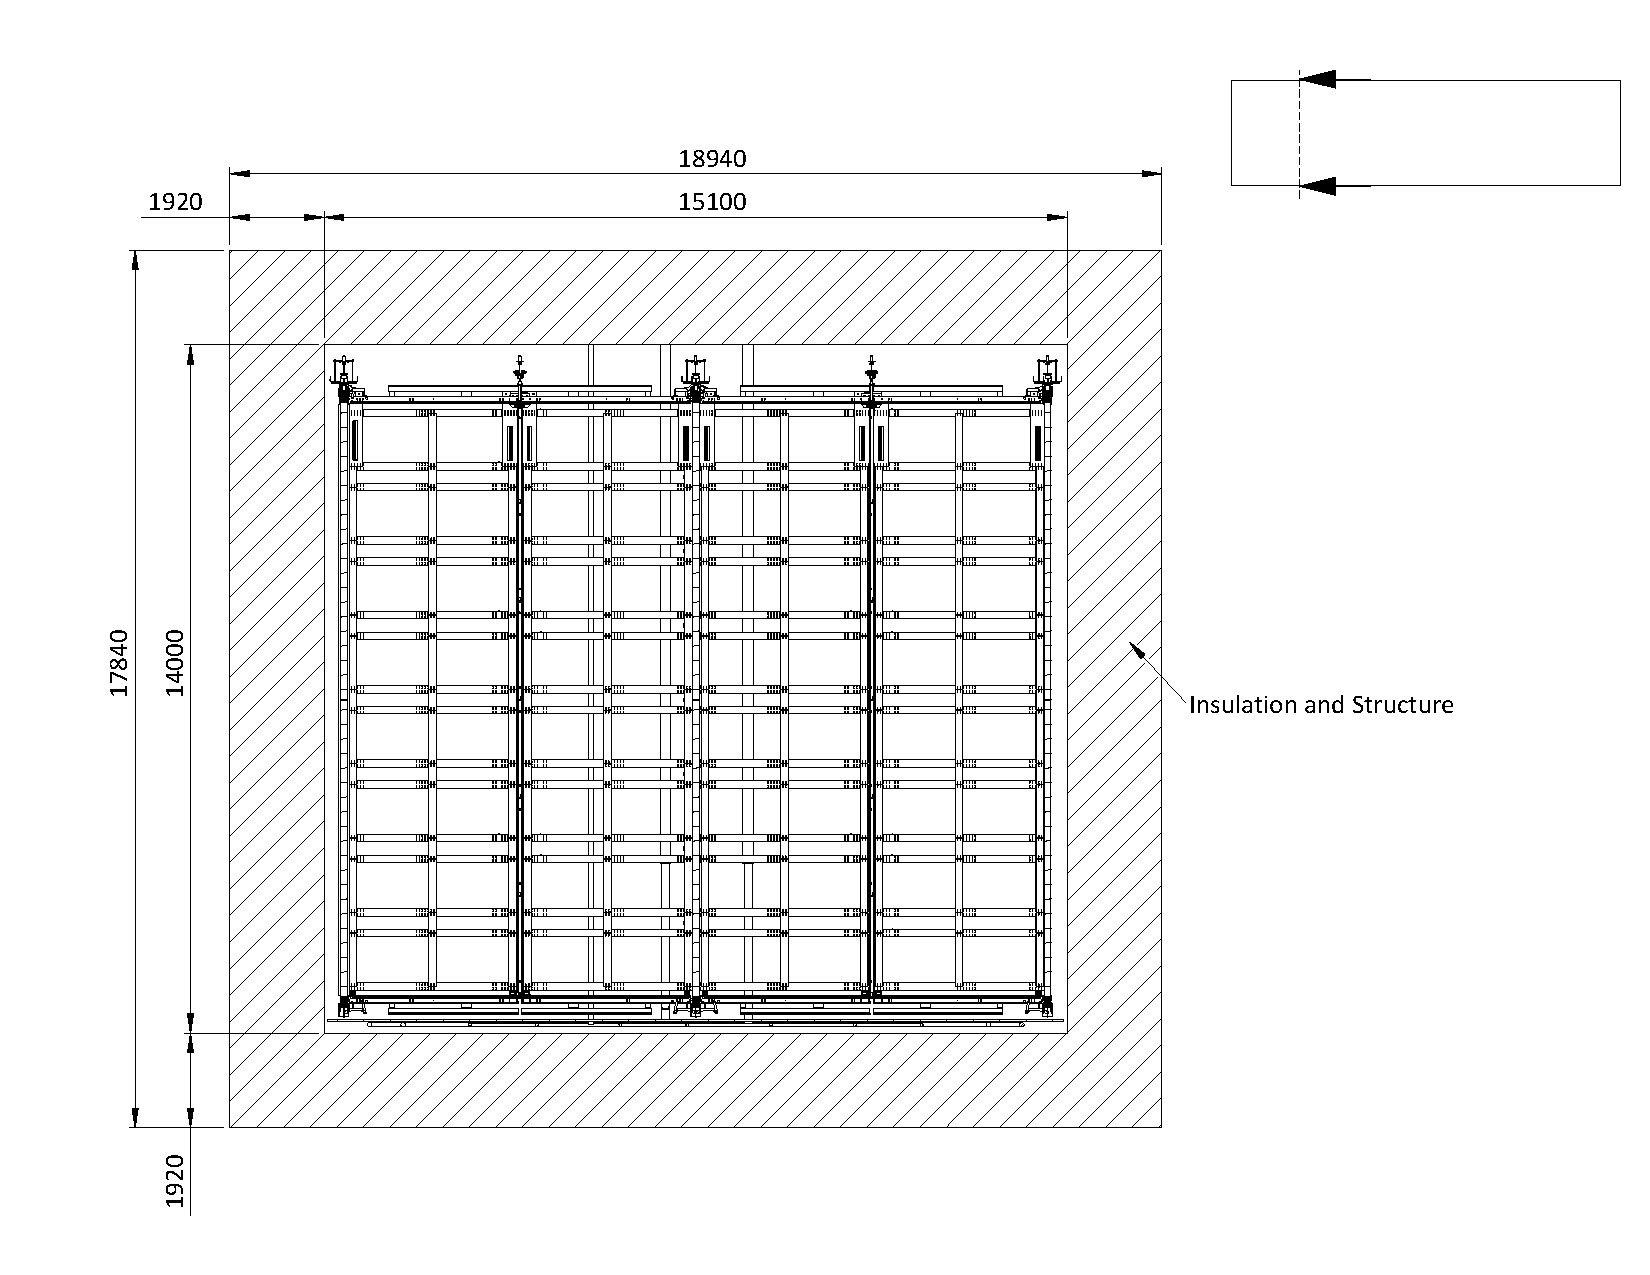
\includegraphics[width=0.65\textwidth]{SP_transverse_section.pdf}
\end{dunefigure}
\begin{dunefigure}[Overall model of the SP module in the
    longitudinal direction]{fig:dune-sp_long}
  {Overall model of the \dword{spmod} in the longitudinal direction.}
  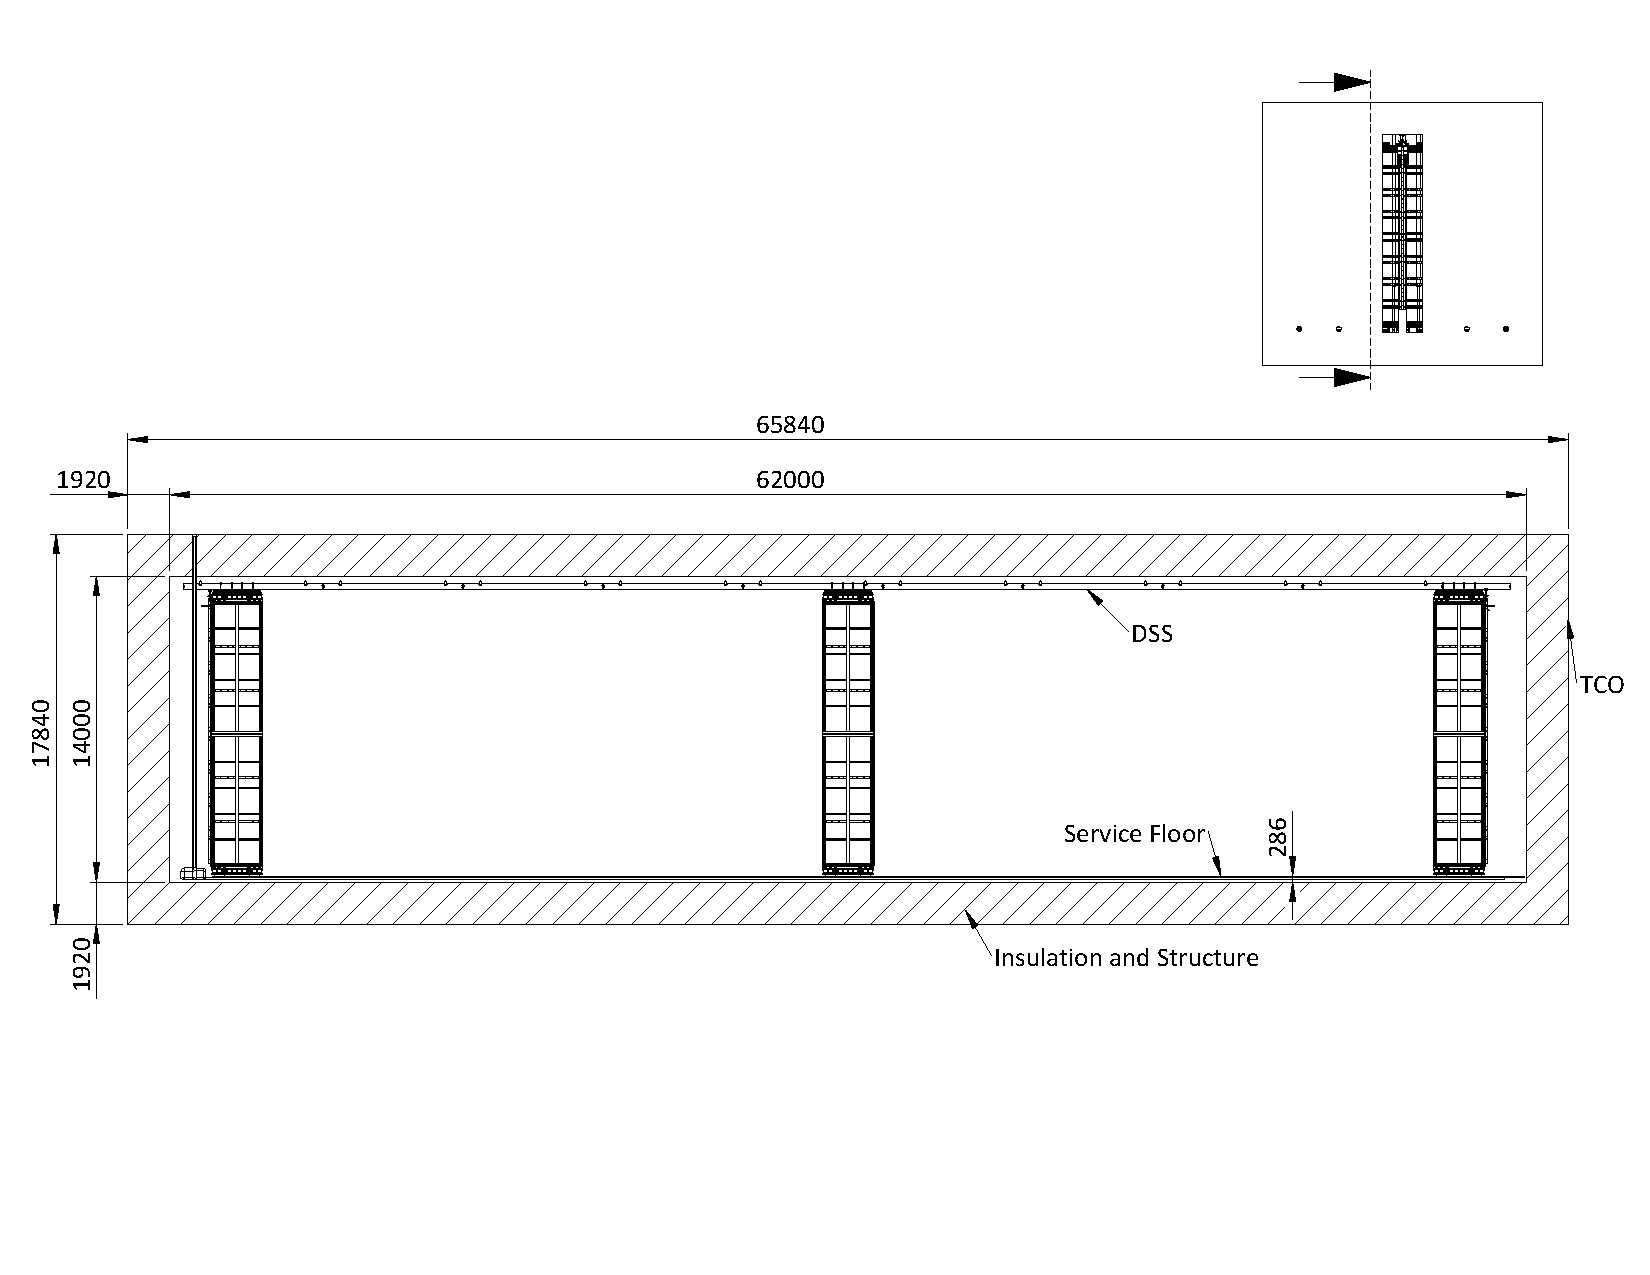
\includegraphics[width=0.85\textwidth]{SP_longitudinal_section.pdf}
\end{dunefigure}



%Figure~\ref{fig:dune-dp_overall} shows the overall model of the \dword{dpmod} with one wall of the cryostat removed to show the interior components. The detector has 20 rows, all of which are constructed the same way. Each row comprises four \dwords{crp}, cathode, \dword{gp}, \dwords{pmt} and side-wall \dwords{fc}.  At the end of row 1 and row 20, \endwall{}s are installed that close the detection volume.
%\begin{dunefigure}[Overall model of the DP module]{fig:dune-dp_overall}
%  {Overall model of \dword{dpmod} .}
%  \fbox{\parbox[c][6cm]{6cm}{
%      \begin{center}
%        Dummy Dual-phase figure
%      \end{center}
%  }}
  %  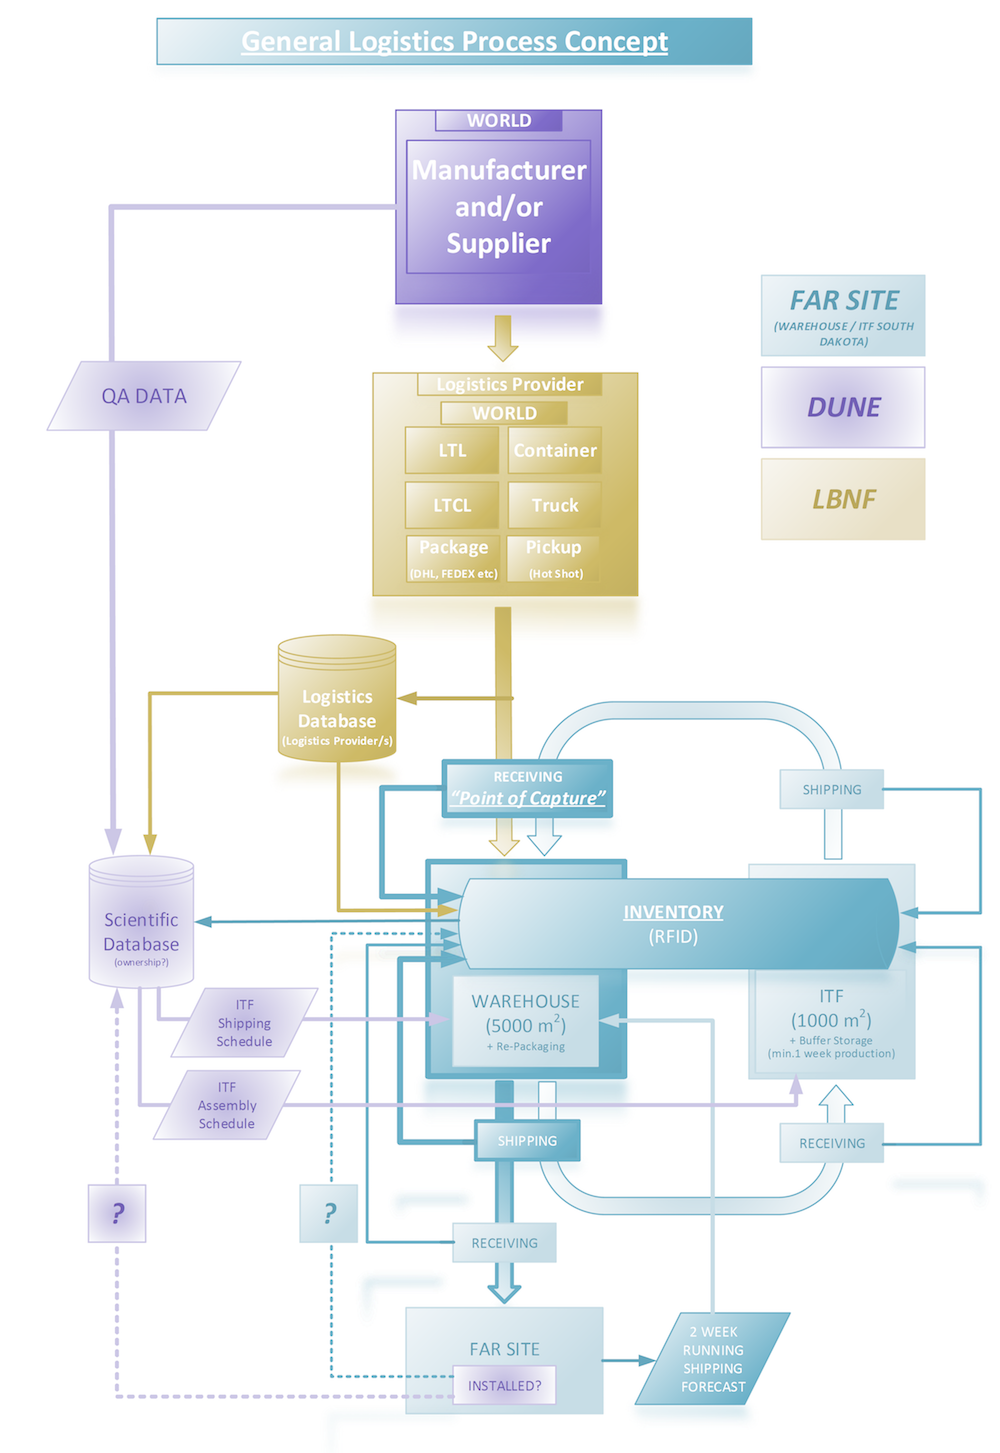
\includegraphics[width=0.85\textwidth]{logistics}
%\end{dunefigure}

\subsection{Envelope and Assembly Models}
\label{sec:fdsp-coord-integ-envelope}

Static models represent the \dword{detmodule} and its components using their exact
design dimensions. Such exact dimensions are needed so that the
detailed component drawings and model remain completely compatible at all
times.


For installation and operation, however, other envelope models are
needed. Envelope models are developed to address issues that affect
installation and operation:
\begin{enumerate}
 \item effects on the detector caused by distortion of the cryostat
   and detector support structure due to gravity;
 \item effects on the detector caused by distortion of the cryostat
   and detector support structure due to loads on the cryostat during
   detector filling and operation;
 \item effects on the detector caused by thermal contraction during
   detector filling and operation;
 \item effects of component and
   assembly tolerances;
 \item clearances needed for installation and envelopes needed for
   access and tooling;
 \item reference models and drawings needed for installation stages
   and to control assembly; and
 \item reference models and drawings needed for alignment and survey.
\end{enumerate}


he models and drawings described above are generated from static
models. Models are also generated to represent combined effects of the
above. In all cases, as with static models, \twod drawings are created
and provide the basis for the installation drawings.


Generating envelope models and drawings are the responsibility of the
\dword{jpo}/\dword{tc} engineering team in coordination with consortia.


\subsection{Integration and Interface Drawings}
\label{sec:fdsp-coord-integ-drawings}

Within each \dword{detmodule}, components from various consortia are
assembled and installed. In addition, components that are the
responsibility of \dword{jpo}/\dword{tc} are assembled and installed in
parallel. The interfaces among components are developed and managed
through models and drawings as described in
Section~\ref{sec:fdsp-coord-integ-models}. Many such interfaces must
be controlled to insure that the detectgor will fit together. The
following section shows some of the interfaces, control drawing,
dimensions, and configurations.


Figure~\ref{fig:dune-apa_interfaces_top} shows the interfaces for the
top \dwords{apa} in the upper corner of the cryostat. It also shows the position
of the cable penetration for the \dword{apa}. Interfaces with cryostat
corrugations and \dword{lar} fill lines are also shown. The reference plane,
defined as the plane of the \dword{apa} yokes, is explained in the
alignment section (Section~\ref{sec:fdsp-coord-integ-survey}).
\begin{dunefigure}[Interface between upper APA,
   FC, cable trays and DSS]{fig:dune-apa_interfaces_top}
  {\dword{spmod} interface between upper \dword{apa}, \dword{fc}, cable
    trays and \dword{dss}.}
  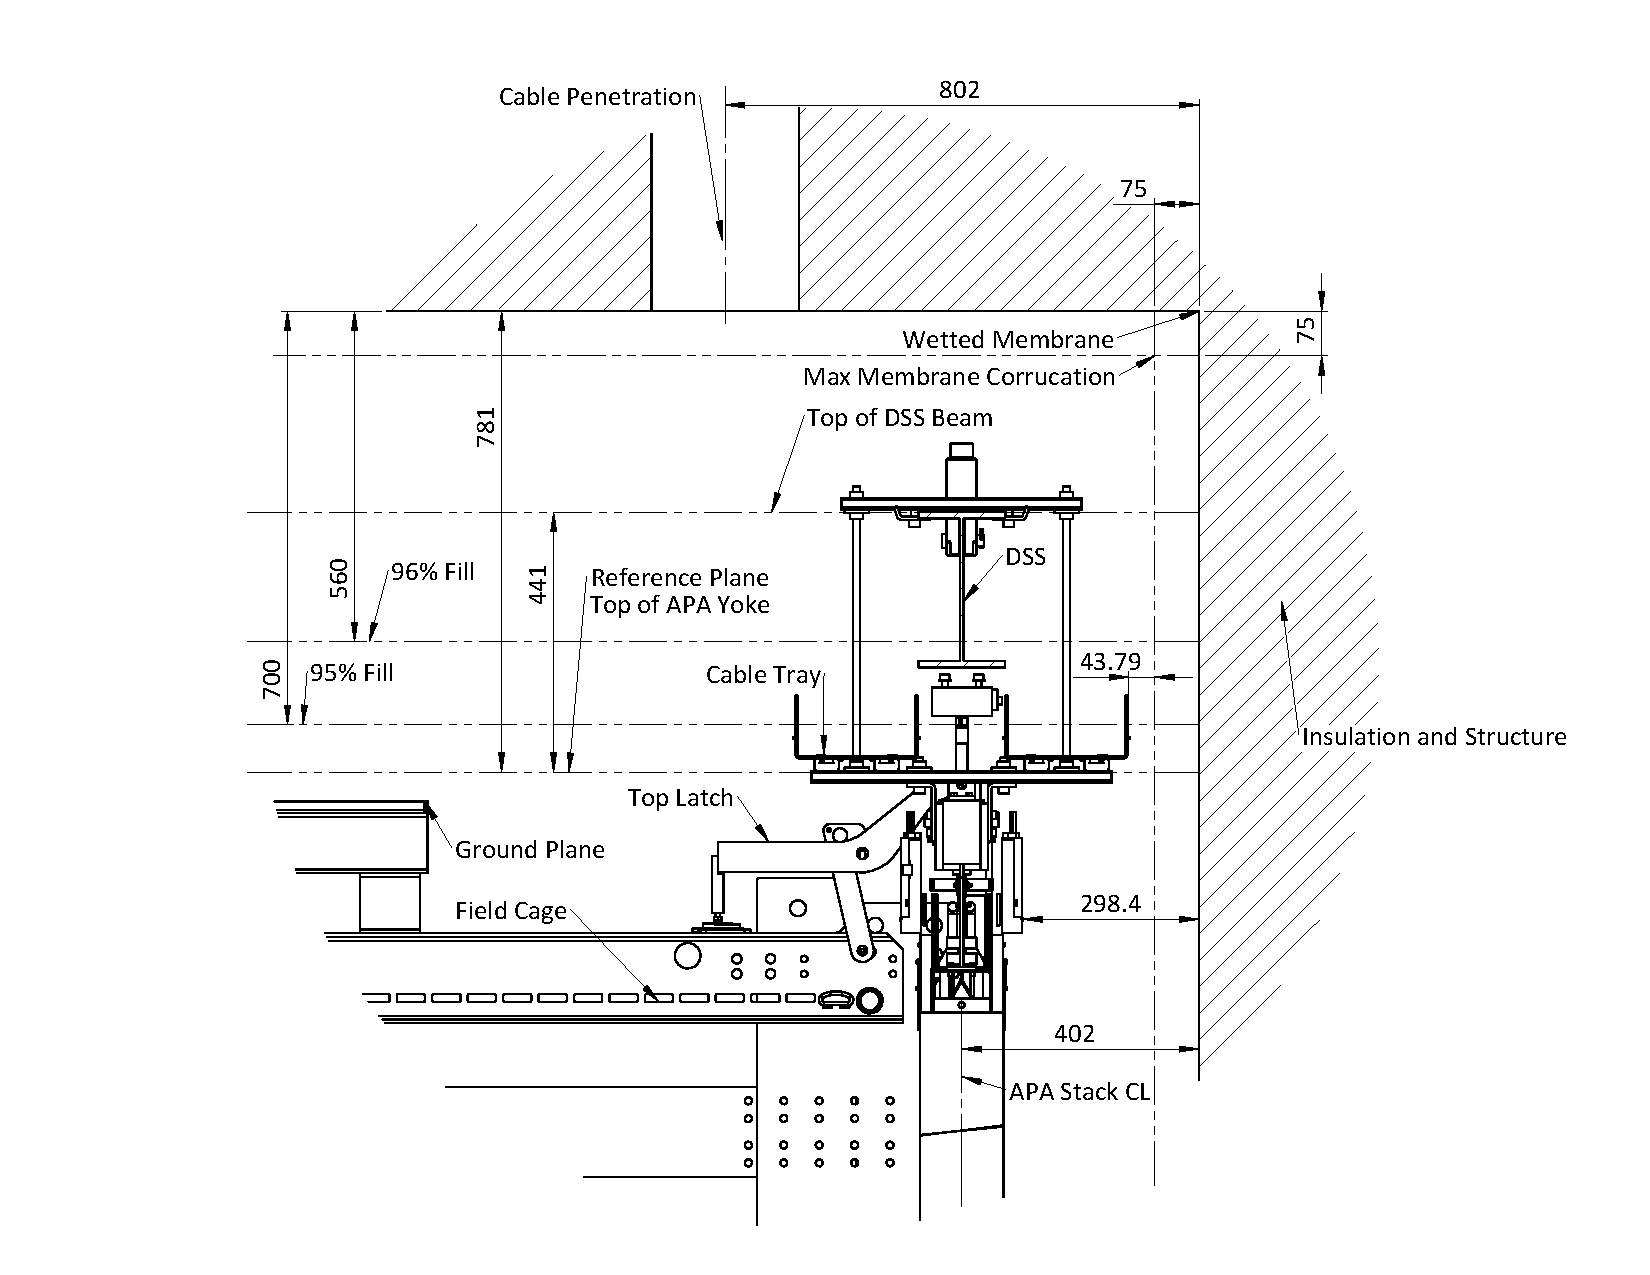
\includegraphics[width=0.8\textwidth]{Interface_upper_apa.pdf}
\end{dunefigure}


Figure~\ref{fig:dune-apa_interfaces_bottom} shows the interfaces for
the bottom \dwords{apa} in the lower corner of the cryostat. In both figures,
the connection latch between the \dwords{fc} and \dwords{apa} is also
shown.
\begin{dunefigure}[Interface between lower APA, FC
    and service floor]{fig:dune-apa_interfaces_bottom}
  {\dword{spmod} interface between lower \dword{apa}, \dword{fc} and
    service floor.}
  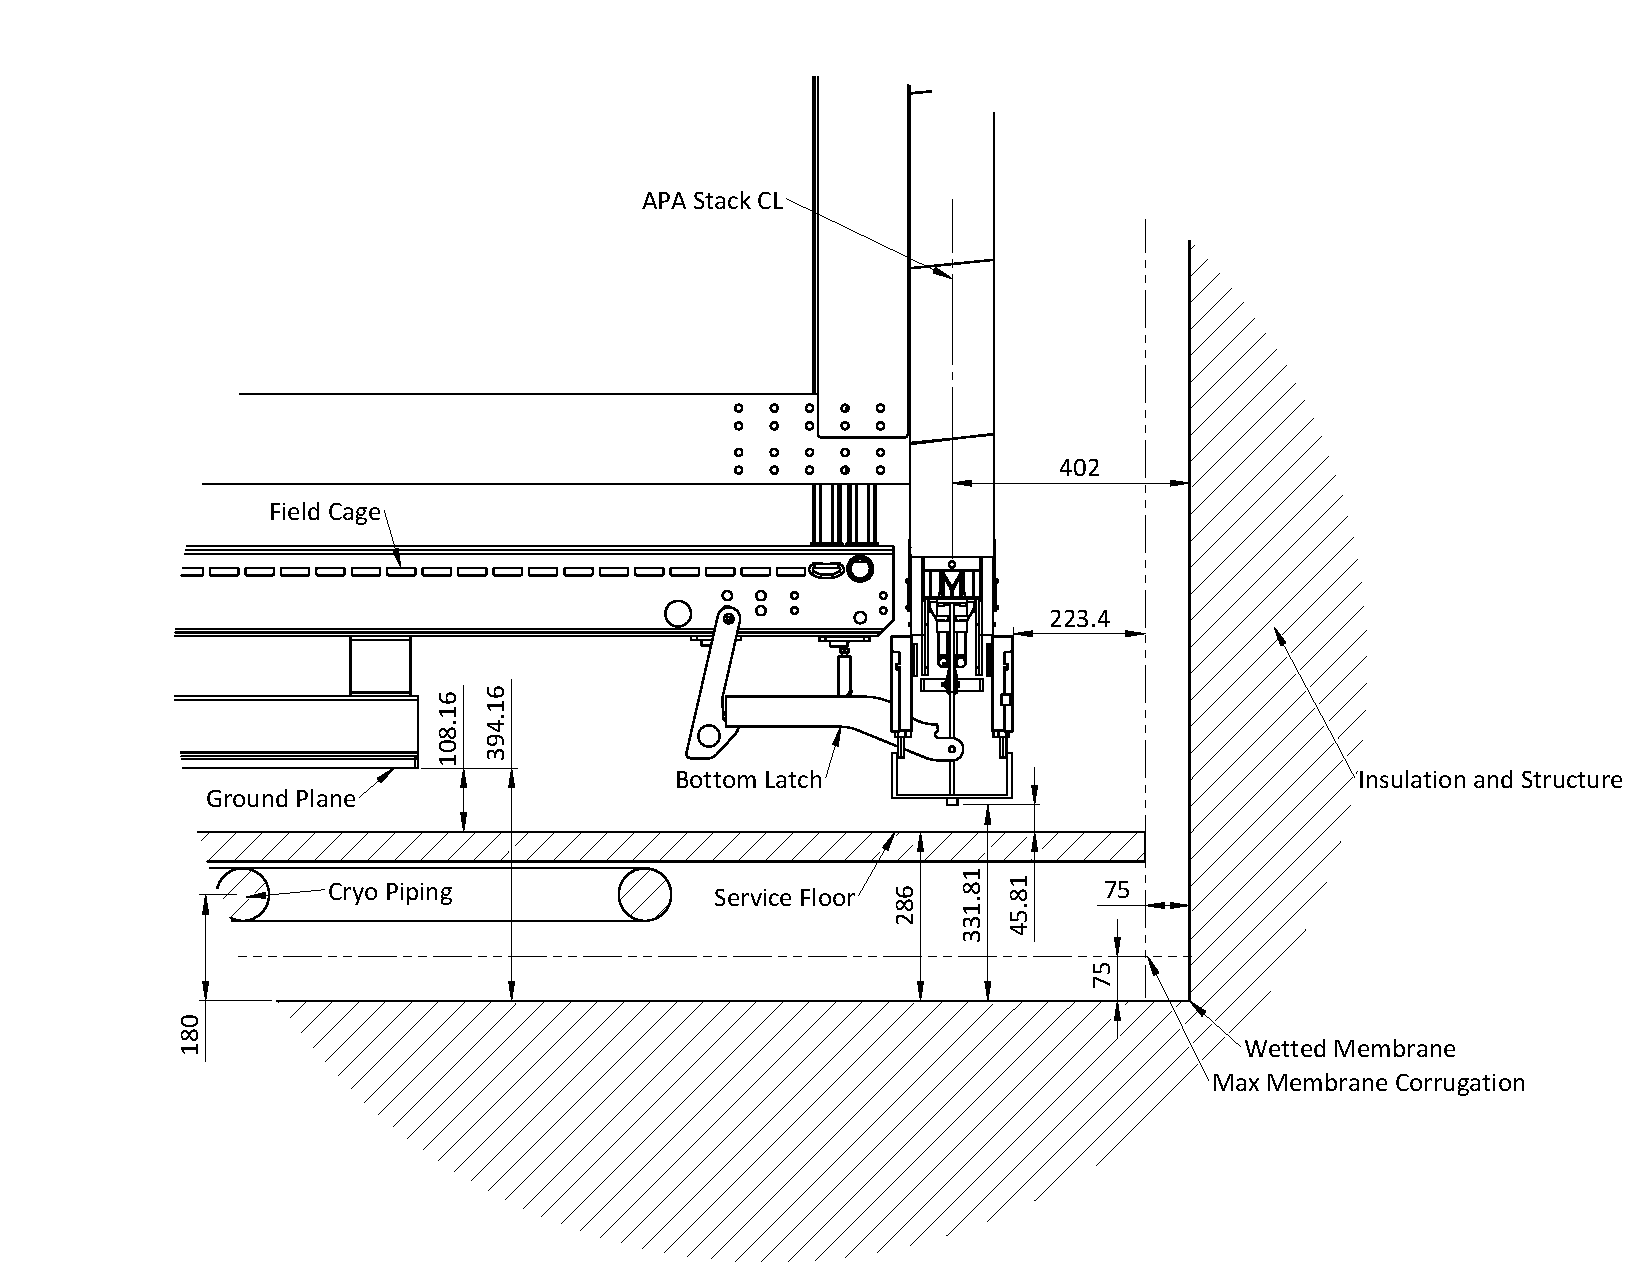
\includegraphics[width=0.7\textwidth]{Interface_lower_apa.pdf}
\end{dunefigure}

Figure~\ref{fig:dune-apa_interfaces_mid} shows the interfaces for the
top of the central row of \dwords{apa} with other components. In this case, a
double latch connection is used. Similarly,
Figure~\ref{fig:dune-cpa_interfaces} shows the interfaces for top of the
\dwords{cpa} with other components.
\begin{dunefigure}[Interface between APA, upper FC
    and GP]{fig:dune-apa_interfaces_mid}
  {\dword{spmod} interface between \dword{apa}, upper \dword{fc} and \dword{gp}}
  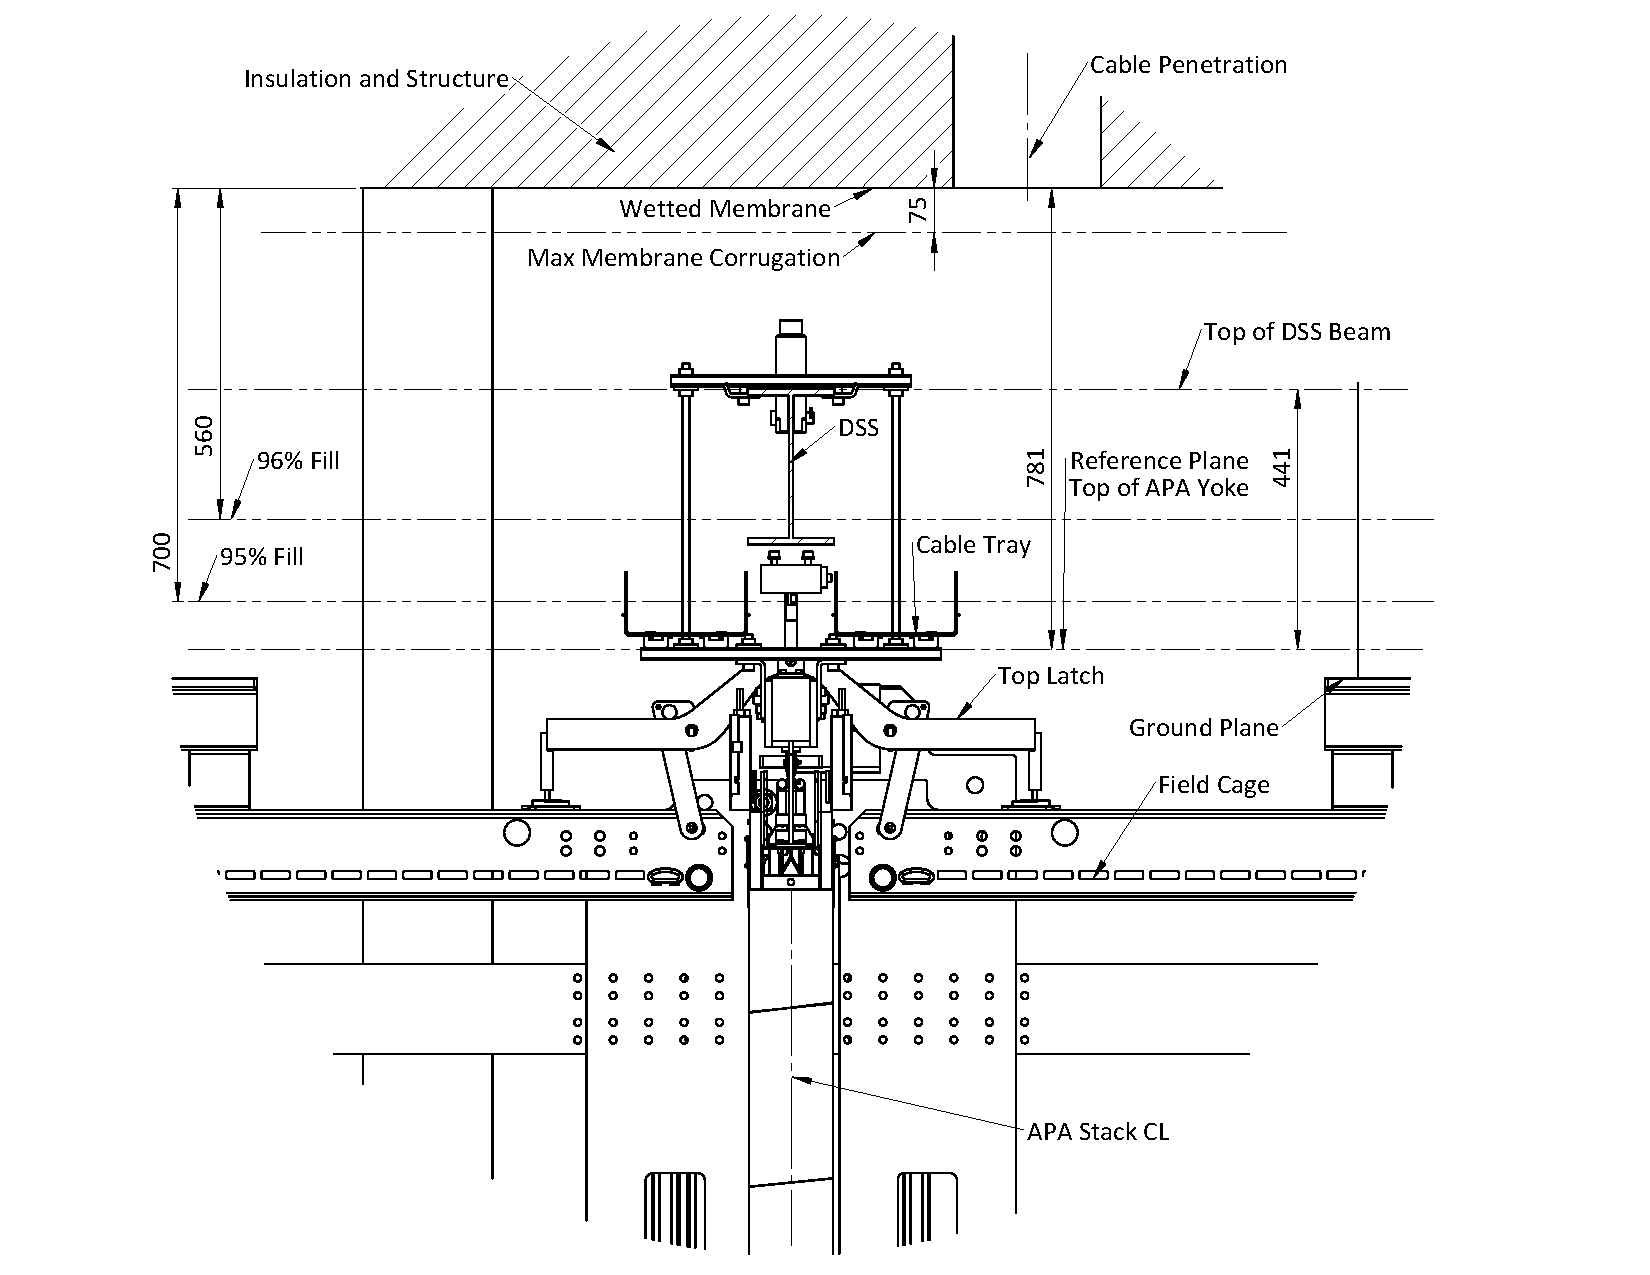
\includegraphics[width=0.8\textwidth]{Interface_upper_mid_apa.pdf}
\end{dunefigure}
\begin{dunefigure}[Interface between CPA, upper FC and GP]
    {fig:dune-cpa_interfaces}
  {\dword{spmod} interface between \dword{cpa}, upper \dword{fc} and \dword{gp}.}
  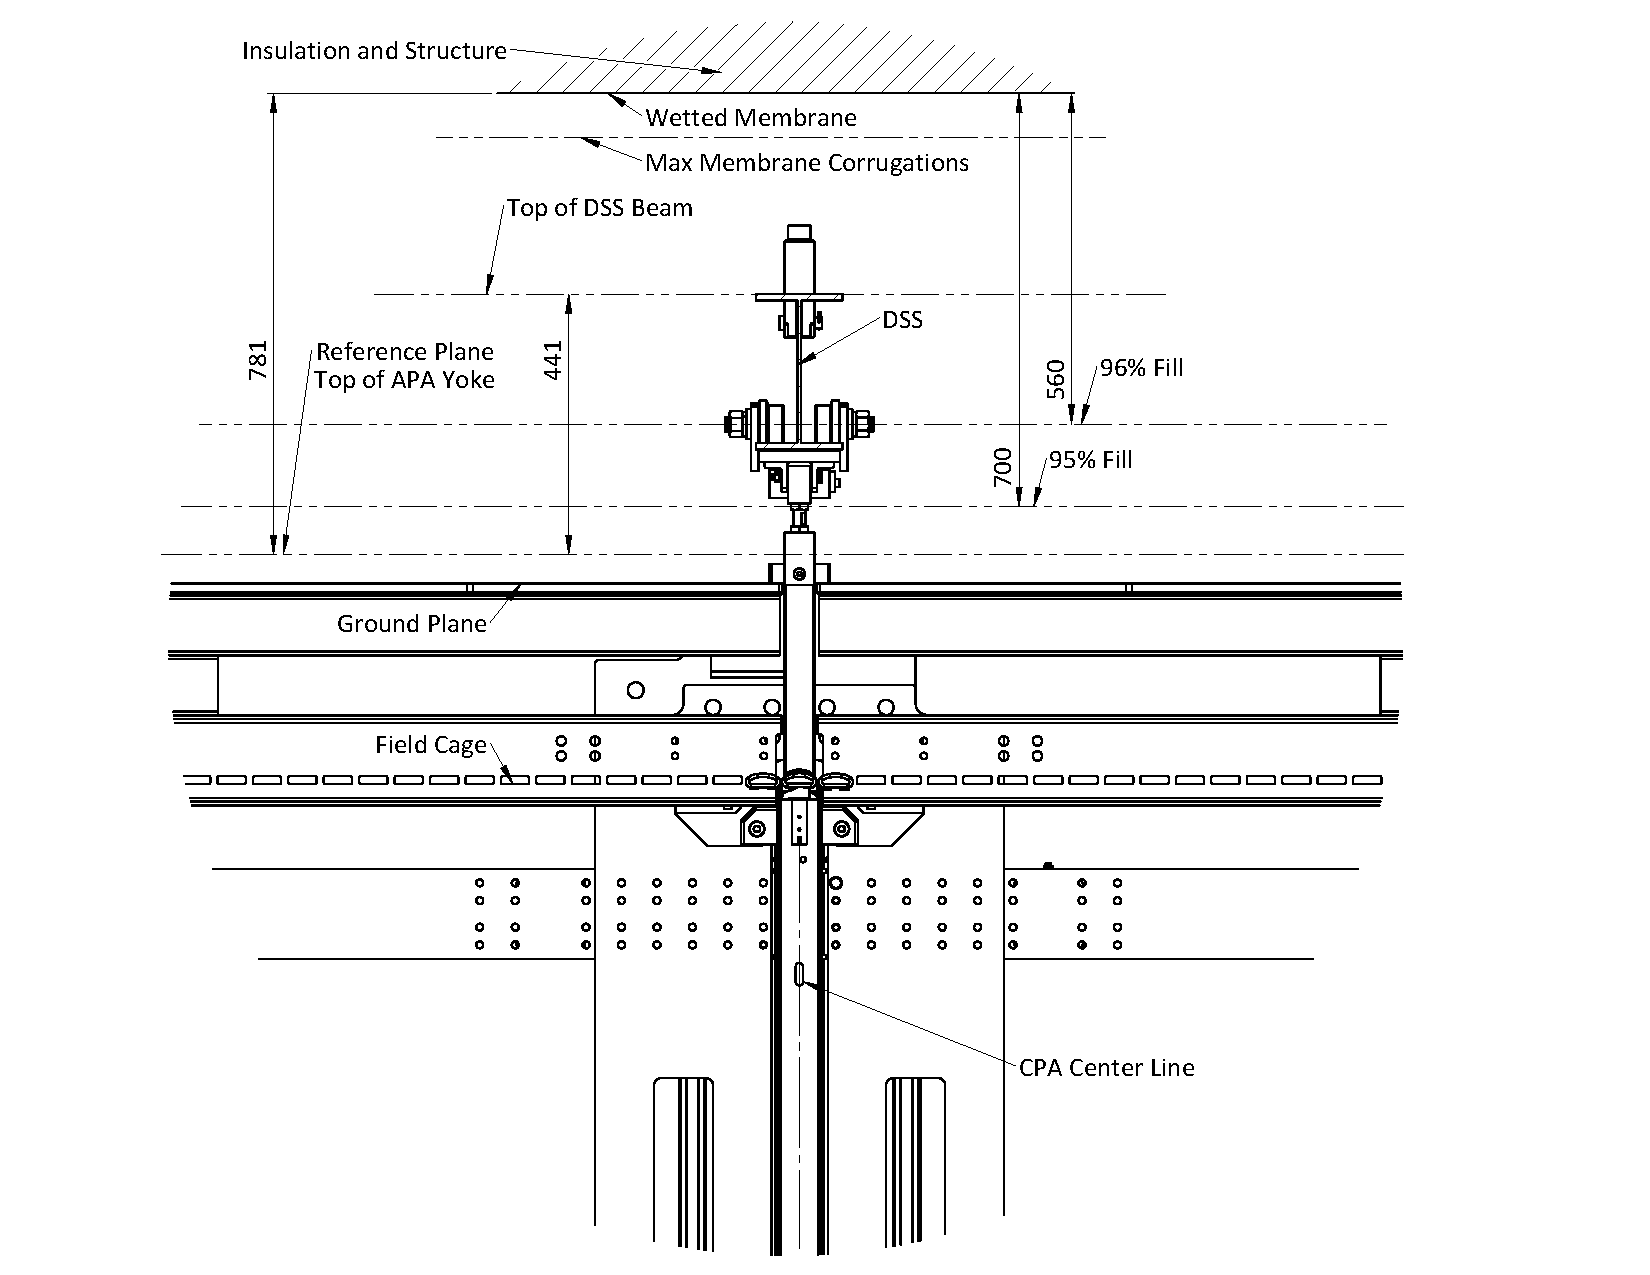
\includegraphics[width=0.8\textwidth]{Interface_upper_cpa.pdf}
\end{dunefigure}

These integration drawings are derived directly from the overall
integration model. The overall integration model is assembled from
component models developed by the consortia. Interfaces are controlled
by \dword{tc}, and consortia maintain their model files to be
compatible with the interfaces. During the design phase, models are
assembled and checked continuously. At the time of final design, all
interfaces will be finalized.


Component tolerances and installation clearances are managed through
additional models as described in
Section~\ref{sec:fdsp-coord-integ-envelope}.
Figure~\ref{fig:dune-apa_envelope} shows the \dwords{apa} and
\dwords{cpa} as well as their relative positions that show how they are
constrained within the detector.
\begin{dunefigure}[Envelope dimensions and
    installation clearances for APAs and CPAs (warm)]
    {fig:dune-apa_envelope} {\dword{spmod} graphical
    representation of envelope dimensions and installation clearances
    for \dwords{apa} and \dwords{cpa} in the warm state.}
  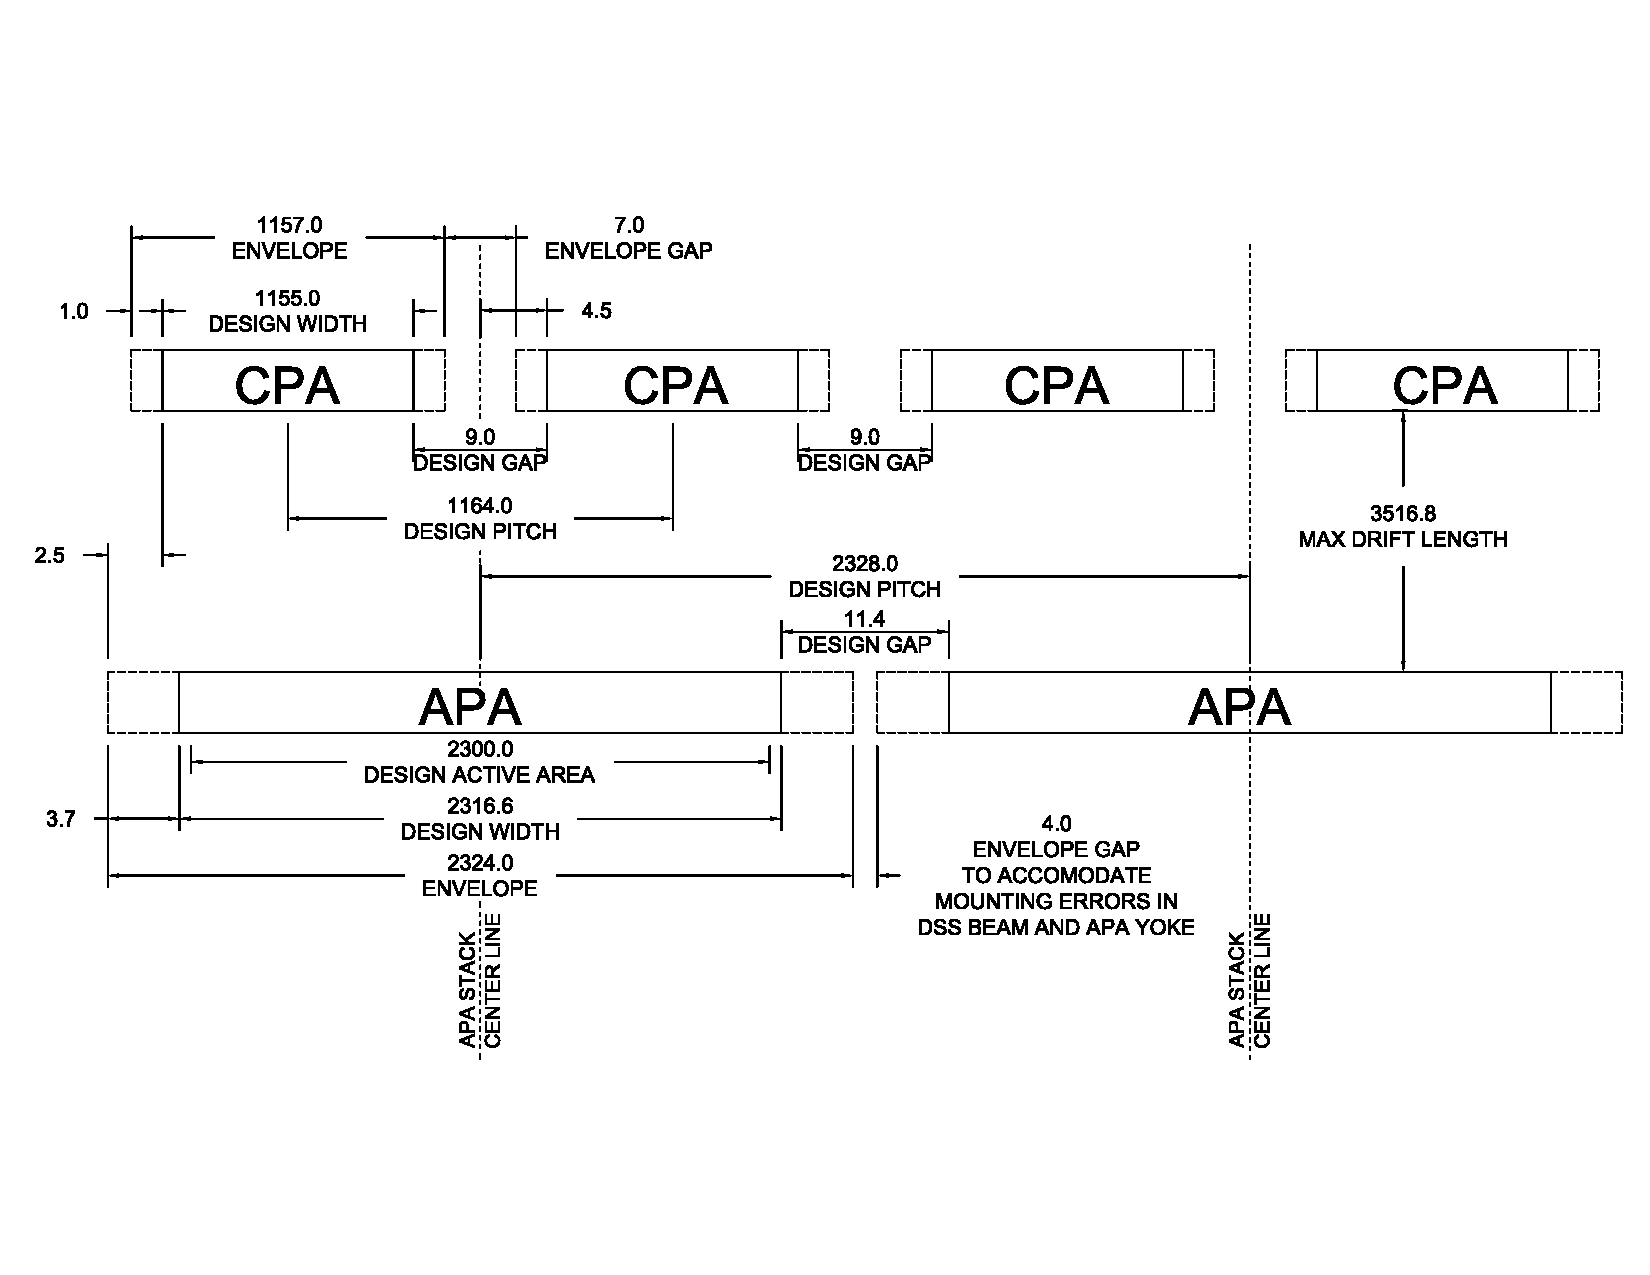
\includegraphics[width=0.95\textwidth]{Warm_envelope_dimensions.pdf}
\end{dunefigure}



Figure~\ref{fig:dune-apa_envelope} shows design dimensions. Component
tolerances and assembly tolerances for the upper and lower
\dword{apa} and \dword{cpa} stacks have been analyzed and are
represented as envelope dimensions. An envelope gap has been defined
to account for tolerances in the support system position and among
components. Taking all of these into account, pitch distances for
\dwords{apa} and \dwords{cpa} have been defined in the warm state.

This figure also shows the design drift distance in the warm
state. The drift distance is defined as the perpendicular distance
between the surface of \dwords{cpa} and the collection wire plane of
\dwords{apa}.

\dwords{apa} and \dwords{cpa} are supported in groups of two or three
on \dword{dss} beams. Fifty beams are arranged into five parallel rows
with 10 beams in each row.  In the cold state, the relative positions
between groups of \dwords{apa} that are supported on different beams
change due to thermal contraction of the beams. Relative positions
within each group supported on the same beam are relatively constant
since \dword{apa} frames and \dword{dss} are both made from stainless
steel.  The effect is that the gap in the active area between some
\dwords{apa} increases.  As can be seen in
Figure~\ref{fig:dune-apa_aa_cold}, in the warm state, the gap in the
active areas between adjacent \dwords{apa} is 28 mm (dotted line). In
the cold state, nine of the 24 gaps increase to approximately 45~mm.
\begin{dunefigure}[APAs active area gap in cold state]{fig:dune-apa_aa_cold} 
    {\dword{spmod} gap in active areas between adjacent \dwords{apa}
      in the cold state. Dashed line warm state, dots cold state.}
    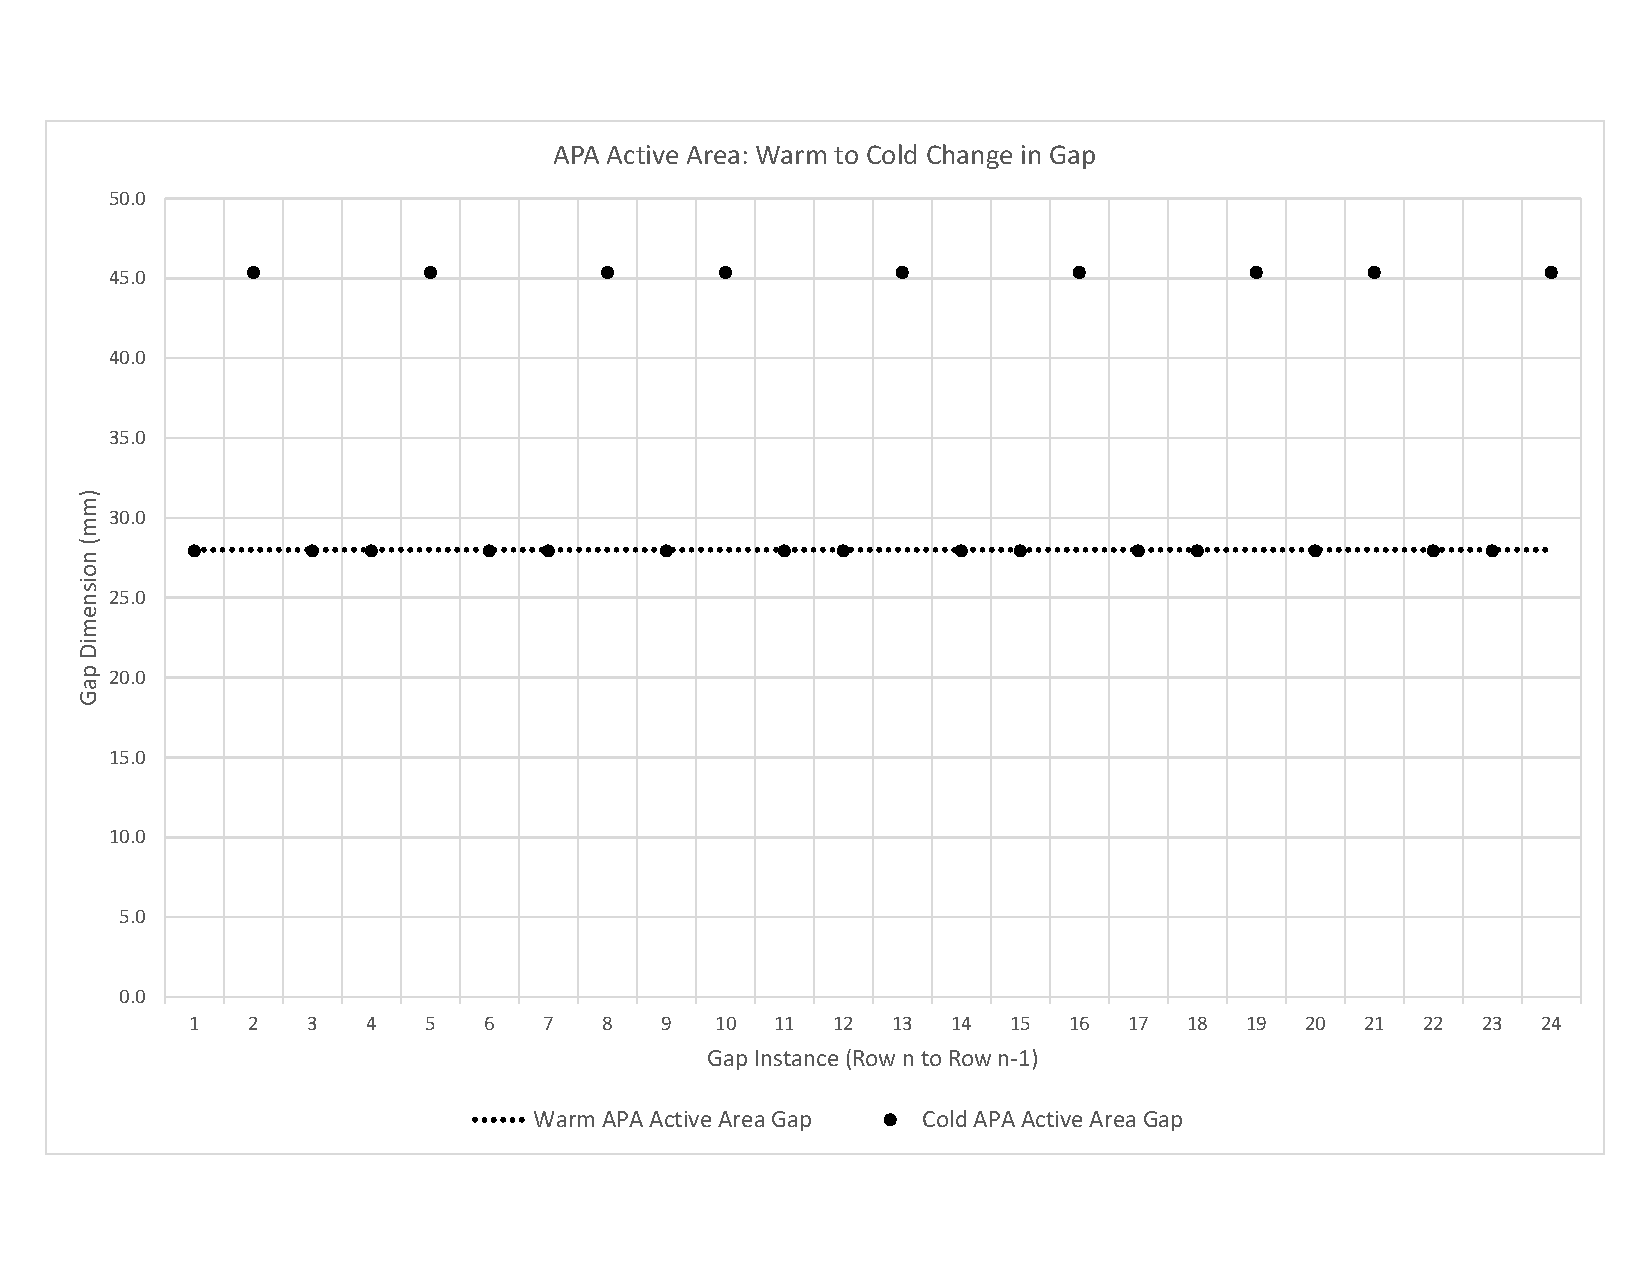
\includegraphics[width=0.8\textwidth]{apa_aa_gap_change.pdf}
\end{dunefigure}

The effects of gravity and buoyancy are not represented in the above
analysis. Such effects are under study and will be shown in the models
as design progresses.

Finally, Figure~\ref{fig:dune-floorpipes} shows the interface of the
cryostat service floor with other components.  Before installing the
\dword{detmodule}, a set of cryogenic distribution pipes are installed
on the floor of the cryostat. These as well as the corrugations of the
cryostat membrane would impede movement, hence the need for
a temporary service floor. It will be installed, and later removed, in sections. 
\begin{dunefigure}[SP module interface of cryogenics, service floor and detector]{fig:dune-floorpipes}
{\dword{spmod} interface of cryogenic distribution pipes, service
  floor, and detector.}
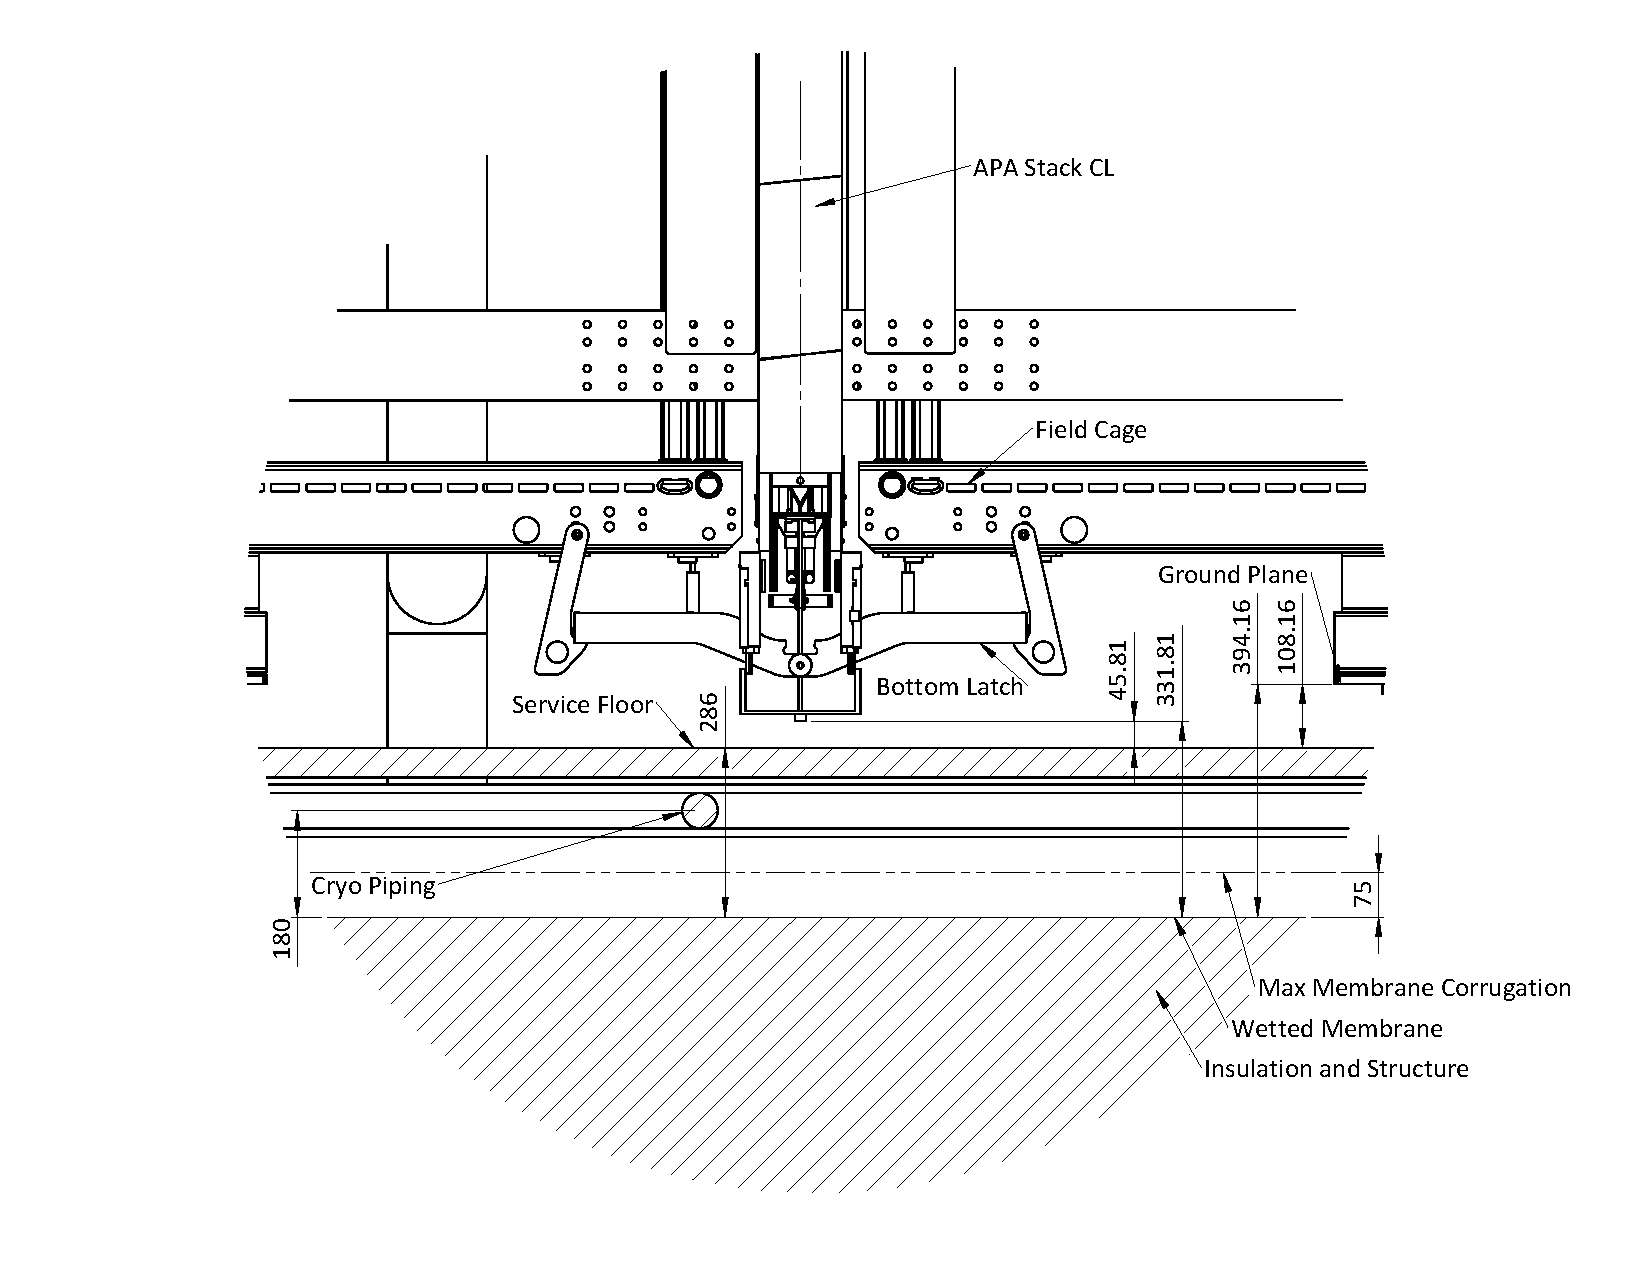
\includegraphics[width=0.8\textwidth]{Interface_lower_mid_apa.pdf}
\end{dunefigure}

\subsection{Detector Survey and Alignment}
\label{sec:fdsp-coord-integ-survey}
The requirement for detector placement within the cryostat is driven
by overall mechanical assembly needs, rather than physics.
Interfacing parts must be assembled properly and function as intended.


In this section, reference frames for the detector are defined so that the
overall survey and alignment can be done within the cavern reference
frame.

For the \dword{spmod}, we define a flat and horizontal reference plane
coplanar with the upper \dword{apa} yoke plane; i.e., 75 yoke planes
define this plane. This reference plane is set at exactly \SI{781}{mm}
below the theoretical plane of the cryostat top membrane.


The detector reference plane is coplanar with the upper \dword{apa}
yoke planes because all features, including the active area, are
referenced to this plane. Once this reference plane is defined and
established through survey, all vertical distances within the detector
are referenced and established relative to it.
Figure~\ref{fig:dune-apa_interfaces_mid} shows the reference plane in
relation to the cryostat top membrane and \dword{dss}.


During installation, the height of the \dword{dss} beams is set in
accordance with this relationship. Adjustments are made in the
\dword{dss} to ensure that all the beams are in the correct plane. The
combined effects of gravity, buoyancy, temperature and \dword{lar}
mass after fill are calculated, and further adjustments are made to
compensate.  This will ensure that the \dword{tpc} position remains as
close as possible to nominal after fill.


The transverse position of the detector is constrained to the center
of the cryostat. Thus, the mid-plane of the middle row \dword{apa} is
coplanar with the vertical mid-plane of the cryostat. This
relationship is verified when the \dword{dss} beams and central row of
\dwords{apa} are installed. The outer rows are similarly aligned and
surveyed with the offset as shown in Figure~\ref{fig:dune-sp_row}.
\begin{dunefigure}[Position of longitudinal
    reference point for the SP module]{fig:dss_feedthru}
  {Position of feedthrough determining the longitudinal reference point of the \dword{spmod}.}
  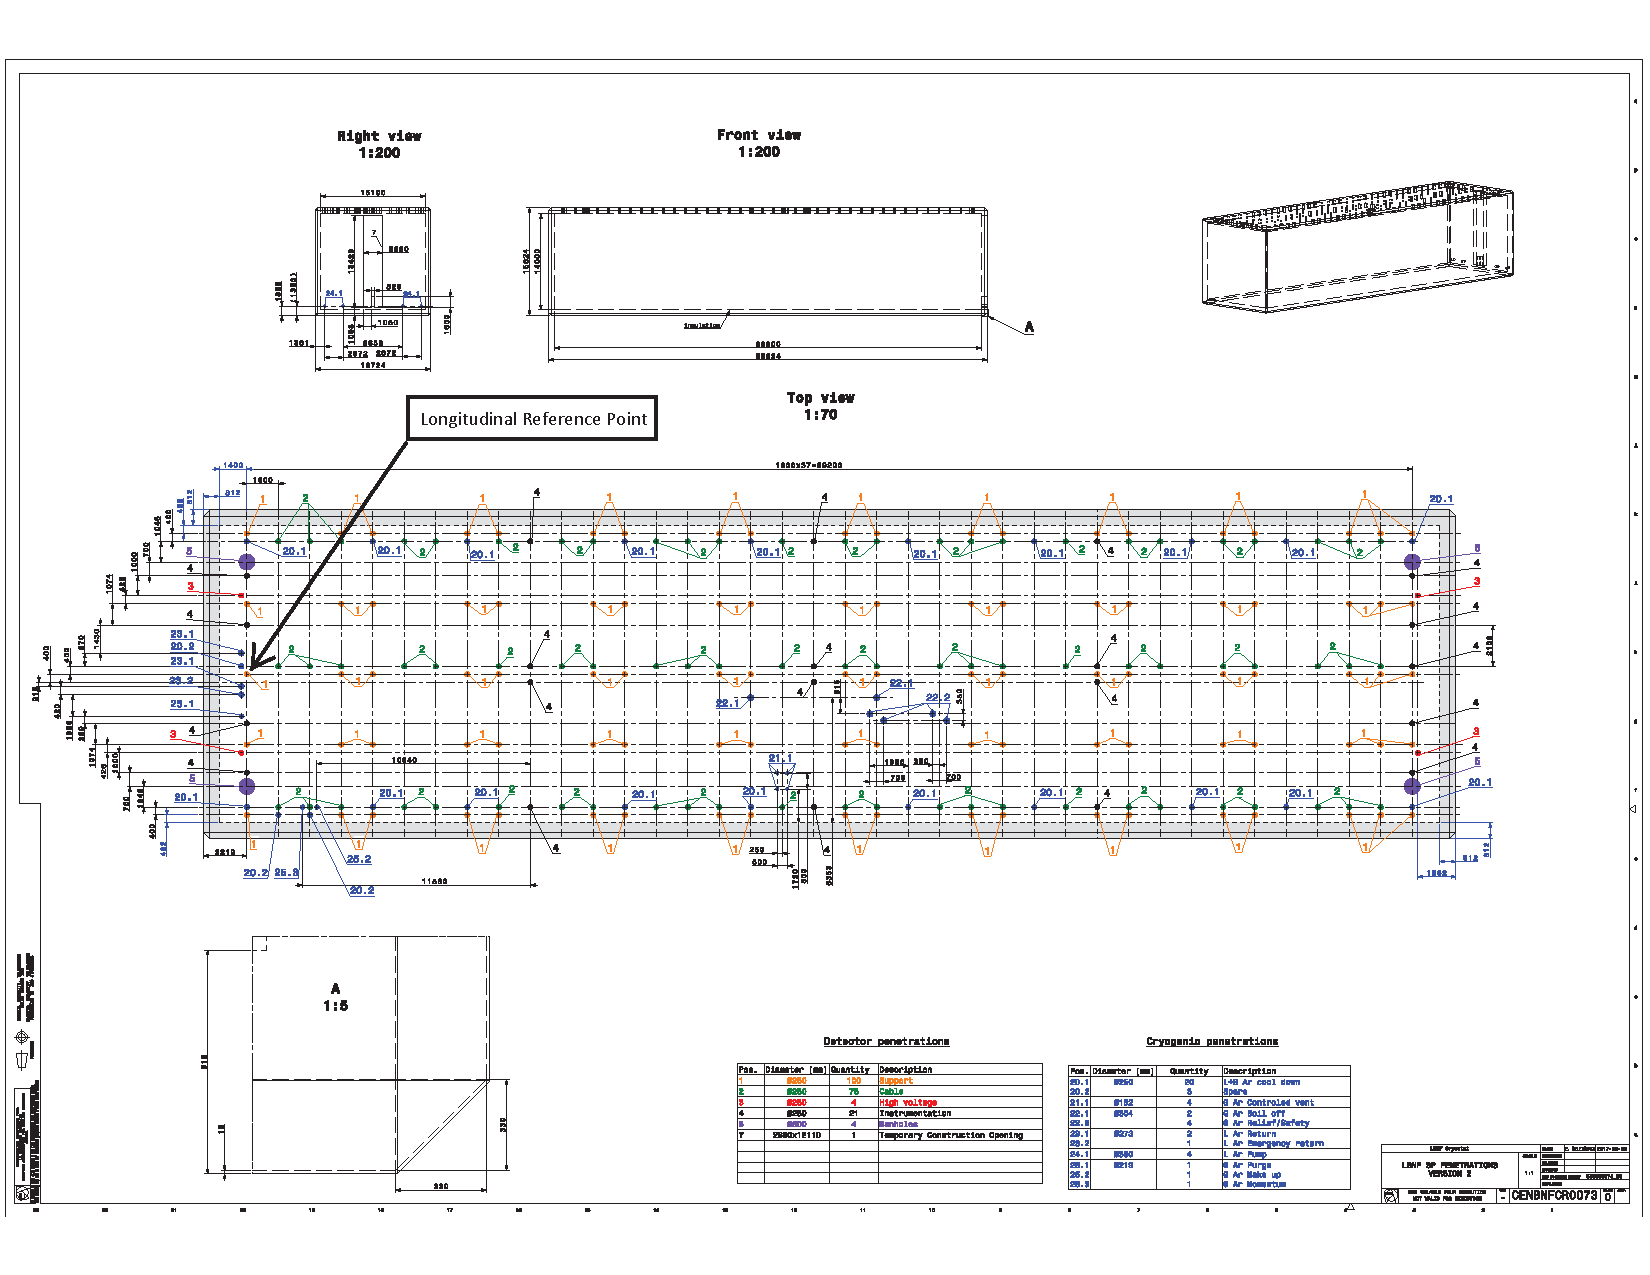
\includegraphics[width=0.9\textwidth]{SP_longitudinal_reference.pdf}
\end{dunefigure}


The longitudinal reference point of the detector within the cryostat
is defined by the position of the single feedthrough of the central row
farthest from the cryostat opening. This feedthrough position
is shown in Figure~\ref{fig:dss_feedthru}.

%\forlbnc{Dual phase should be similar transversely and longitudinally; vertically, it needs to be determined}


\section{Electrical Integration}
\label{sec:fdsp-Integ-electrical}


\subsection{Electrical System Block Drawings, Schematics, Layouts and Wiring Diagrams}
\label{sec:fdsp-coord-electrical}


\dword{jpo}/\dword{tc} is responsible for the AC power distribution supplied to
the experiment and to detector electronics racks.  This is described
in Sections~\ref{sec:fdsp-coord-faci-grounding}
and~\ref{sec:fdsp-coord-faci-power}.  Specific guidance has been
provided regarding the use of DC power supplies and cable shield
treatment.  These guidelines are specified in
EDMS-2095958\cite{bib:cernedms2095958}. They are the same as were
followed at \dword{protodune} and developed during extensive testing
of the \dword{apa} wire readout at \dword{bnl} and \dword{protodune}.
Guidelines are included for the treatment of DC power supplies and the
use and connection of shielded cables.  All systems are reviewed for
compliance to these guidelines during the design review procedure.
Any deviation from the guidelines must be noted and approved by system
engineering.

\dword{tc} will review all electrical systems to ensure that they
follow safe design practice and will pass \dwords{orr} as discussed in
Chapter~\ref{vl:tc-review}.  Review by \dword{tc} will include vetting
of all power and ground paths, adherence to national electrical
standards or equivalents for all commercial equipment, and adherence
to the \dword{dune} electrical design rules.

The electrical design of each subsystem is described by a set of
documents that includes a system-level block diagram and a wiring
diagram that includes a complete description of all power and ground
connections.  Depending on what is being described, a complete set of
schematics, board production files and wiring diagrams will be
reviewed and archived.  All designs are subject to electrical safety
review, as described above, before production proceeds. The safety
reviews proceed in conjunction with the overall review process as
described in Chapter~\ref{vl:tc-review}.

Consortia will produce system-level block diagrams. The \dword{tcoord}
will ensure that these diagrams are produced and reviewed.  In some
cases, multiple diagrams may be required, e.g., the \dword{cisc}
consortium is responsible for several types of systems (such as
temperature readouts, purity monitors, cameras, pressure sensors),
each requiring a separate diagram. A system-level block diagram should
show the conceptual blocks required in the design along with
connections to other conceptual block elements, both inside and
outside the given consortium.
Figure~\ref{fig:electrical_blockdiagram_example} shows an example of a
system-level block diagram.
\begin{dunefigure}[Sample system-level block diagram]{fig:electrical_blockdiagram_example}
  {Electrical system-level block diagram example (\dword{spmod} \dword{ce}).}
 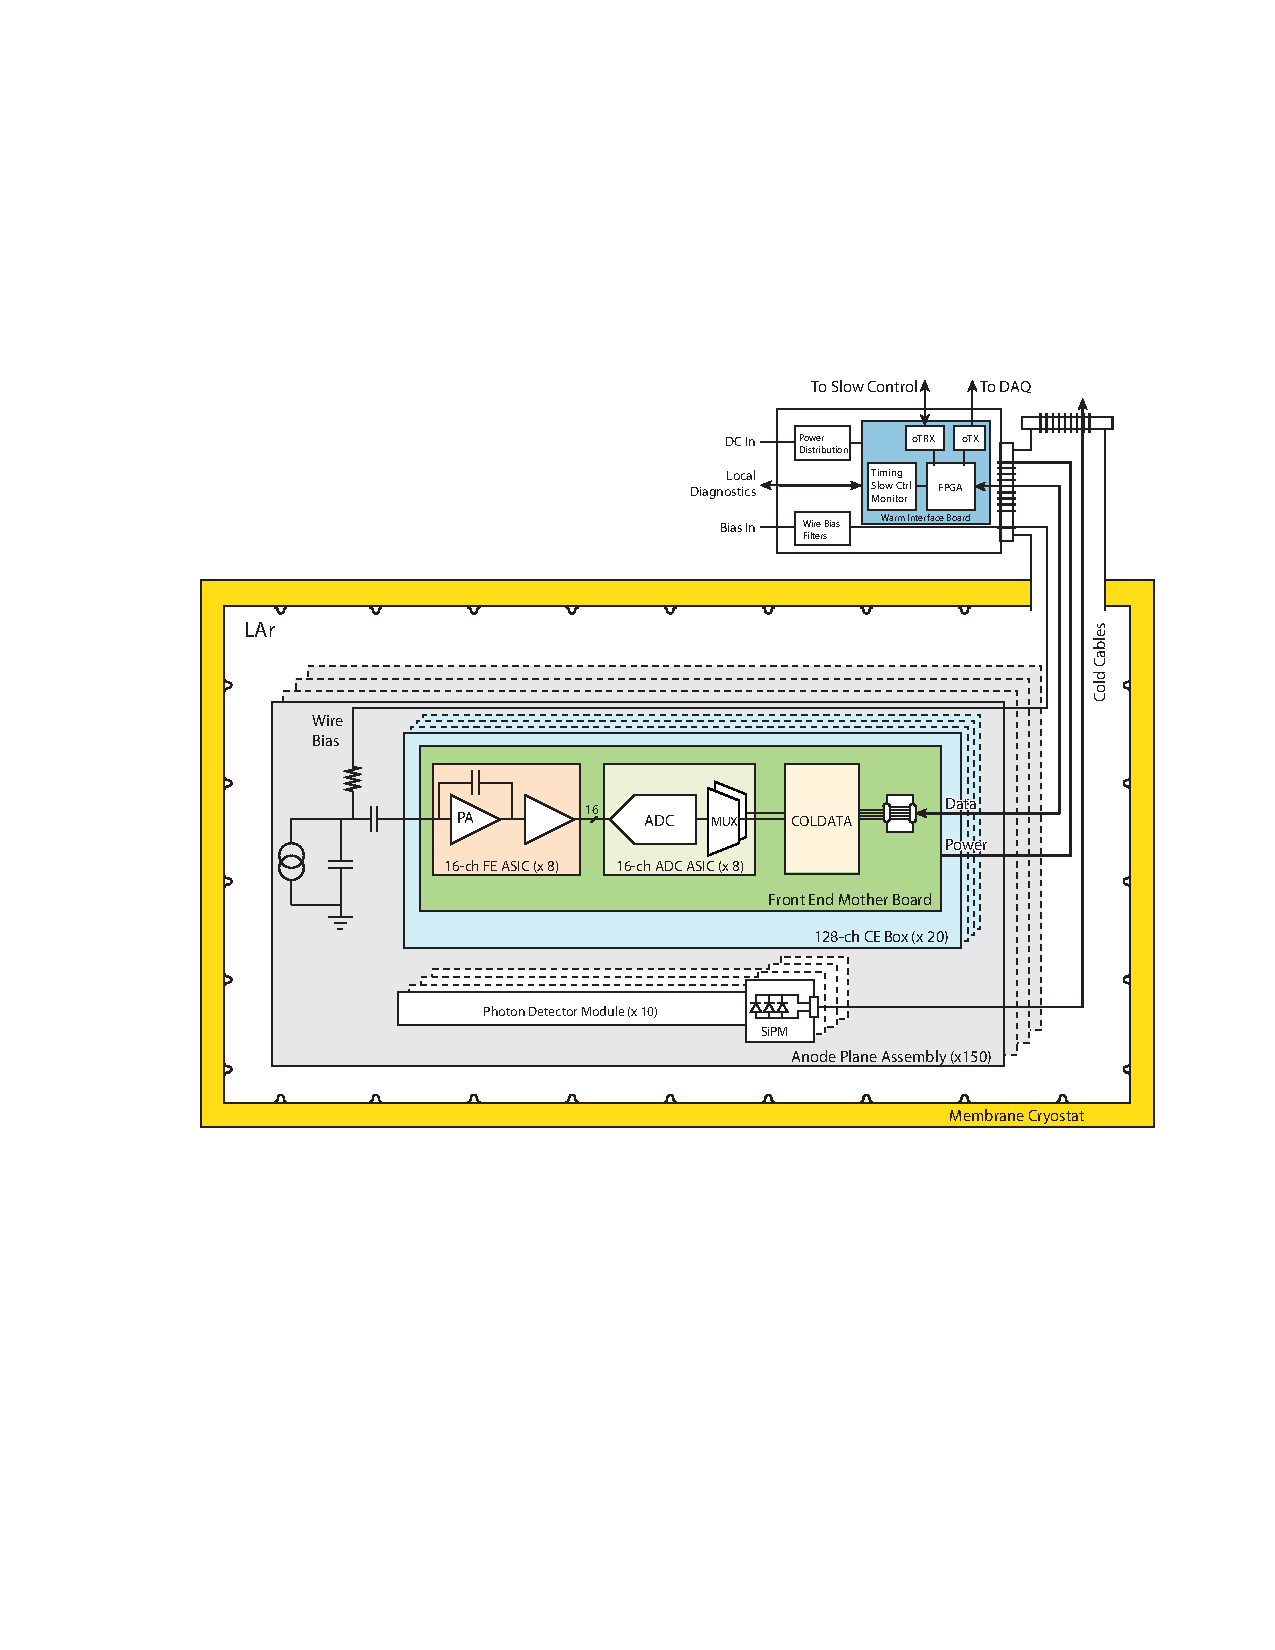
\includegraphics[width=0.85\textwidth]{Example_System_Level_Block-Diagram-SP_Cold_Electronics.pdf}
\end{dunefigure}


All consortia must provide an electrical wiring diagram that 
represents the power and ground distribution within the system being
described.  The paths of power and ground distribution wiring between
circuit elements are specified along with wire types and sizes.  Power
elements like power supplies, fuses (or other protective circuit
elements), power connectors, and pin and wire ampacity are documented.


Electrical schematics show very specifically how individual
components are connected.  Usually, a schematic will represent a
\dword{pcb} design.  Schematics call out specific
parts that are used in the design and include all interconnections.
In the case of a \dword{pcb}, layout files, manufacturing
specifications, and bills of materials document
the design and allow a safety review of any custom boards or
modules.


Wiring diagrams include all wire and cable connections that run
between \dwords{pcb} or electronics modules.  Wires and
cables are described within the diagram and include identification of
\dword{awg}, wire color, cable specification and
cable connectors and pinouts.


\subsection{Electrical Integration Documentation}
\label{sec:fdsp-coord-integ-electrical}

%Section~\ref{sec:fdsp-coord-electrical} lists the documentation a consortium must provide to describe construction of a subsystem for which it is responsible.
Interfaces that occur between subsystems of different consortia will
be documented and formally agreed upon between the technical leads of
the coordinating consortia and must be verified by the \dword{tc}
team.  Much of the documentation required to describe a subsystem can
be used for the interface documents.

Documentation required for the interface between two electrical
subsystems includes a block diagram that identifies all connections
between the subsystems.  This block diagram must exist in the formal
interface document between consortia.  For each connection, additional
documentation must fully describe the interface details. This
additional detailed information can exist outside of the primary
interface document between the consortia, but that document must point
to it.


A signal cable that runs between \dwords{pcb} belonging to different
consortia is an example of an integration interface.  For a signal
cable, interface documentation includes the connector specifications,
pinouts at each end of the cable, and the pinout of the board
connectors.  Documentation would also describe relevant electrical
signal characteristics that may include signal levels, function,
protocol, bandwidth and timing information.  If different subsystems
refer to a given signal by different names, documentation of signal
name cross reference must be provided.

Consortium technical leads and the \dword{tc} team sign off
and approve the detailed documentation information on integration
interfaces not included in the primary consortium-to-consortium
interface document.

The \dword{tc} team will provide unique names and labels
for all racks, crates, boards, power supplies, cables and any other
electrical type equipment.  A database will be created to track these
devices.

\section{Configuration and Drawing Storage and Dissemination}
\label{sec:fdsp-coord-integ-modelplan}

The consortia and \dword{jpo}/\dword{tc} engineering team create and share
drawings, models, schematics, production data and all other
engineering documents. In addition, the \dword{jpo}/\dword{tc} engineering team
generates and shares all interface drawings and documentation.

Folders have been set up to allow uploading and sharing documents
with appropriate protection. The structure of the folders has been set
up to suit each consortium. The consortia do not necessarily have
similar folder structures or files, and will adapt the structure to fit
their needs.

The folders and files reside on the \dword{edms}. This system and
similar structures were used for \dword{protodune} and are being
used by \dword{lbnf}.

The following shows a high-level outline of the file structure. The
first section is for technical coordination files. The second
section is generic, intended for a consortium. Each consortium will have one such
folder.
\begin{enumerate}
 \item \dword{jpo}/\dword{tc}
 \begin{enumerate}
  \item mechanical drawings and files (controlled by \dword{dune} lead mechanical engineer)
  \begin{enumerate}
    \item \dword{fd} general drawings for illustration (controlled by \dword{tcoord})
    \item \threed model files of internal detector for periodic upload to global model
    \item \twod interface drawing files
    \item alignment and survey files
    \item Ash River installation test facility files
    \item \dword{qa}/\dword{qc} files
    \item safety analysis and documentation
    \item design reviews
  \end{enumerate}
  \item electrical and electronics (controlled by lead electrical engineer of \dword{dune})
  \begin{enumerate}
    \item infrastructure requirements for grounding
    \item consortium interface drawings
    \item detector electronics grounding guidelines
    \item detector safety system
    \item \dword{qa}/\dword{qc} files
    \item safety analysis and documentation
      \item design reviews
  \end{enumerate}
 \end{enumerate}
 \item consortium files (one per consortium, controlled by consortium technical leads)
 \begin{enumerate}
   \item \threed model files
   \item \twod part drawing files
   \item production files
   \item general grounding diagrams
   \item system level block diagrams
   \item system level wiring diagrams
   \item software and firmware plans
   \item custom components, such as \dwords{asic} (one folder per component)
   \item \dword{pcb} components (one folder per component)
   \item cable components (one folder per component)
   \item power supply components (one folder per component)
 \end{enumerate}
\end{enumerate}
An image of the \dword{edms} file structure is shown in
Figure~\ref{fig:config_structure}.
\begin{dunefigure}[\dword{edms} file structure]{fig:config_structure}
  {\dword{edms} file structure}
  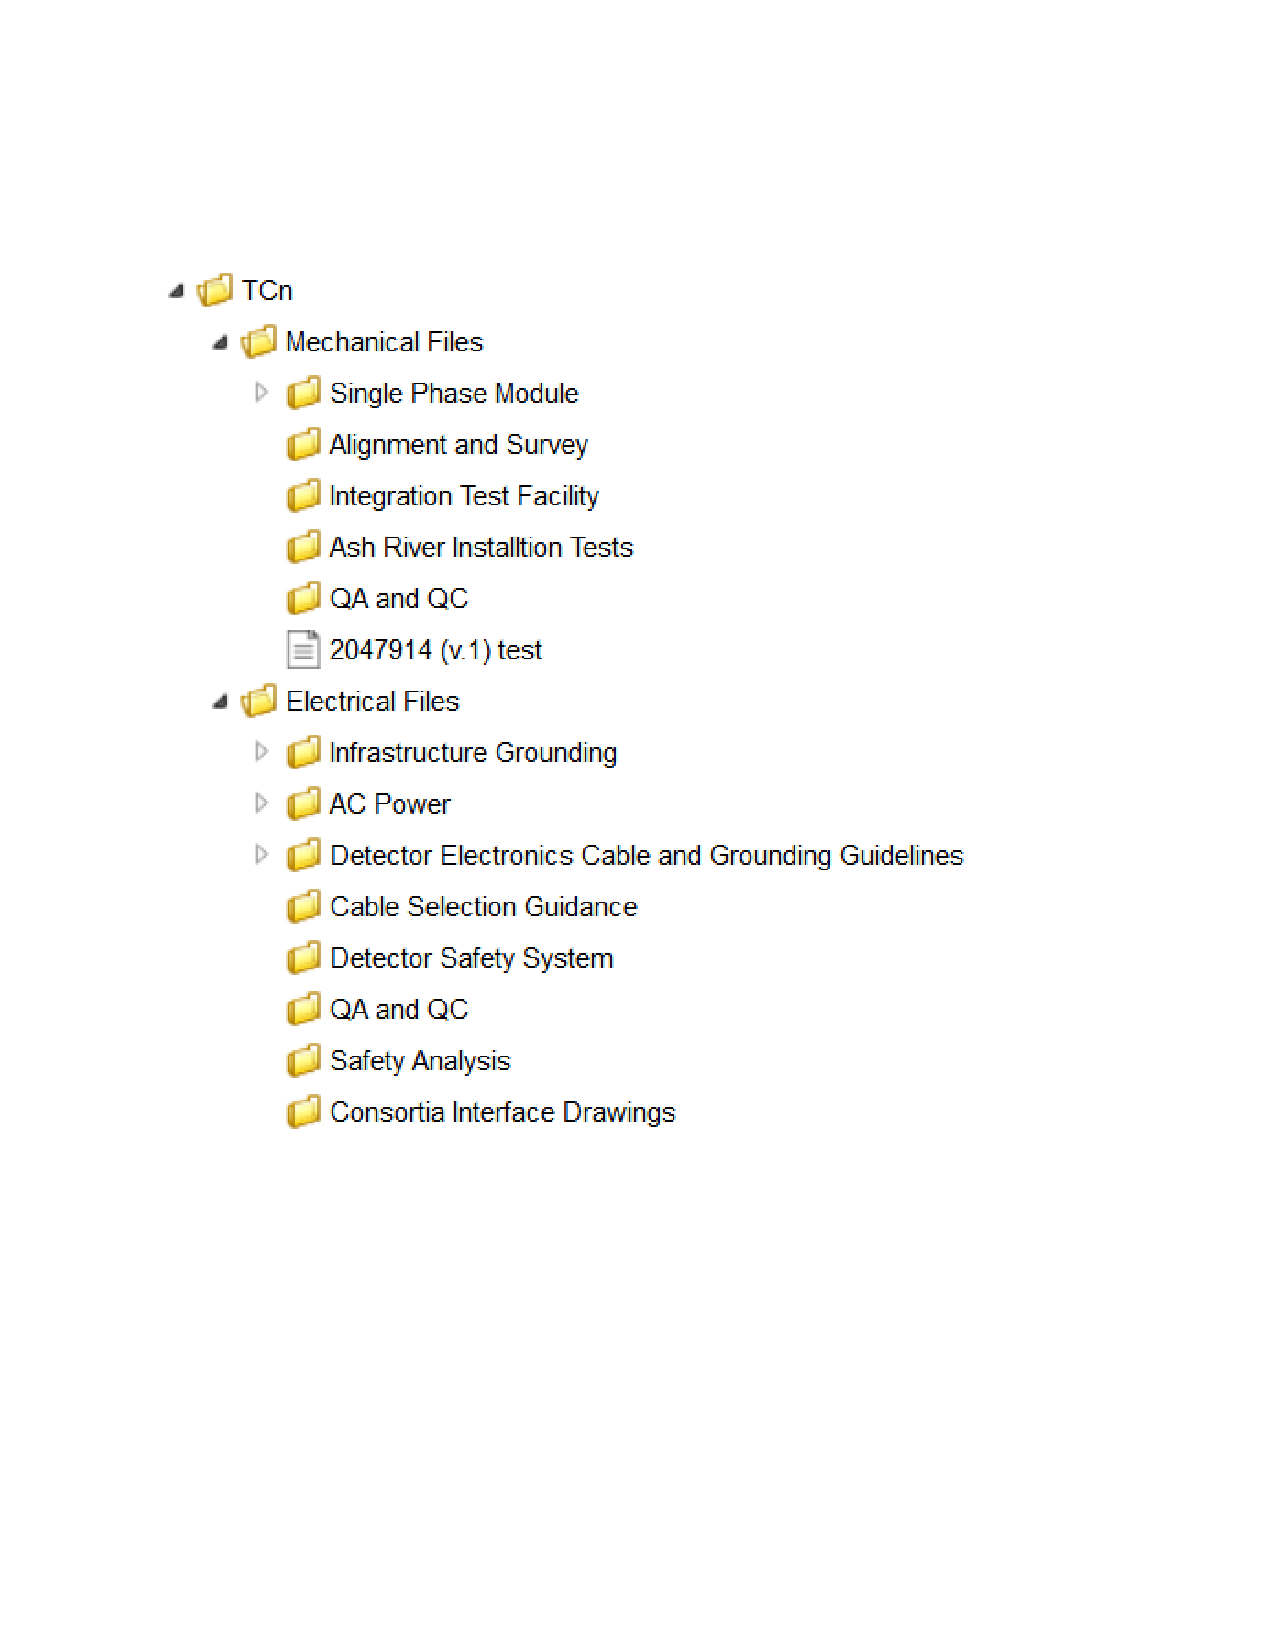
\includegraphics[width=0.5\textwidth]{config_storage_v2}
\end{dunefigure}

\section{Organization of Interfaces and Interface Documents}
\label{sec:fdsp-coord-integ-interface}

An integration mechanism has been developed to manage and create an
overall model of interfaces both within a \dword{detmodule} and
between a \dword{detmodule} and facilities, The mechanism defines
integration nodes, which can be thought of as focus areas, as
explained below.  The \dword{jpo}/\dword{tc} engineering team carries out and
manages interfaces between the nodes. The integration nodes comprise the following:
\begin{itemize}
\item {\bf Detector:} This consists of all \dword{tpc} elements within
  the \dword{lar}. Almost all consortia are involved in this
  integration task, which is mostly mechanical. Consortium engineering
  teams work directly with the \dword{tc} engineering team.  The
  primary interface is with \dword{dss} through hangers. Examples of
  interfaces within this node include: \dword{fc} connections to both
  \dwords{cpa} and \dwords{apa}, \dword{ce} and \dword{pd} cable
  routing within the cryostat, and location of calibration and
  cryogenics instrumentation.
\item {\bf \dword{dss}:} This consists of all detector support elements,
  cable trays and feedthroughs.
\item {\bf Detector Electronics:} This consists of all racks, cooling,
  power, cable trays, cable distribution on top of the cryostats, rack
  protection (smoke detectors, hardware power trip), rack component
  build and the interface to the \dword{ddss}.
\item {\bf \dword{daq} and electronics:} This includes electronics on
  top of the cryostat, in the \dword{daq} room and in the surface
  rooms. This also includes the fiber optic distribution from the
  surface to the \dword{daq} room and the fiber optic distribution
  from the \dwords{detmodule} to the \dword{daq} room. It also includes the
  layout and cooling of the \dword{daq} room.
\end{itemize}

\begin{dunefigure}[Integration Nodes]{fig:integration_nodes}
  {Overall integration nodes and interfaces}
  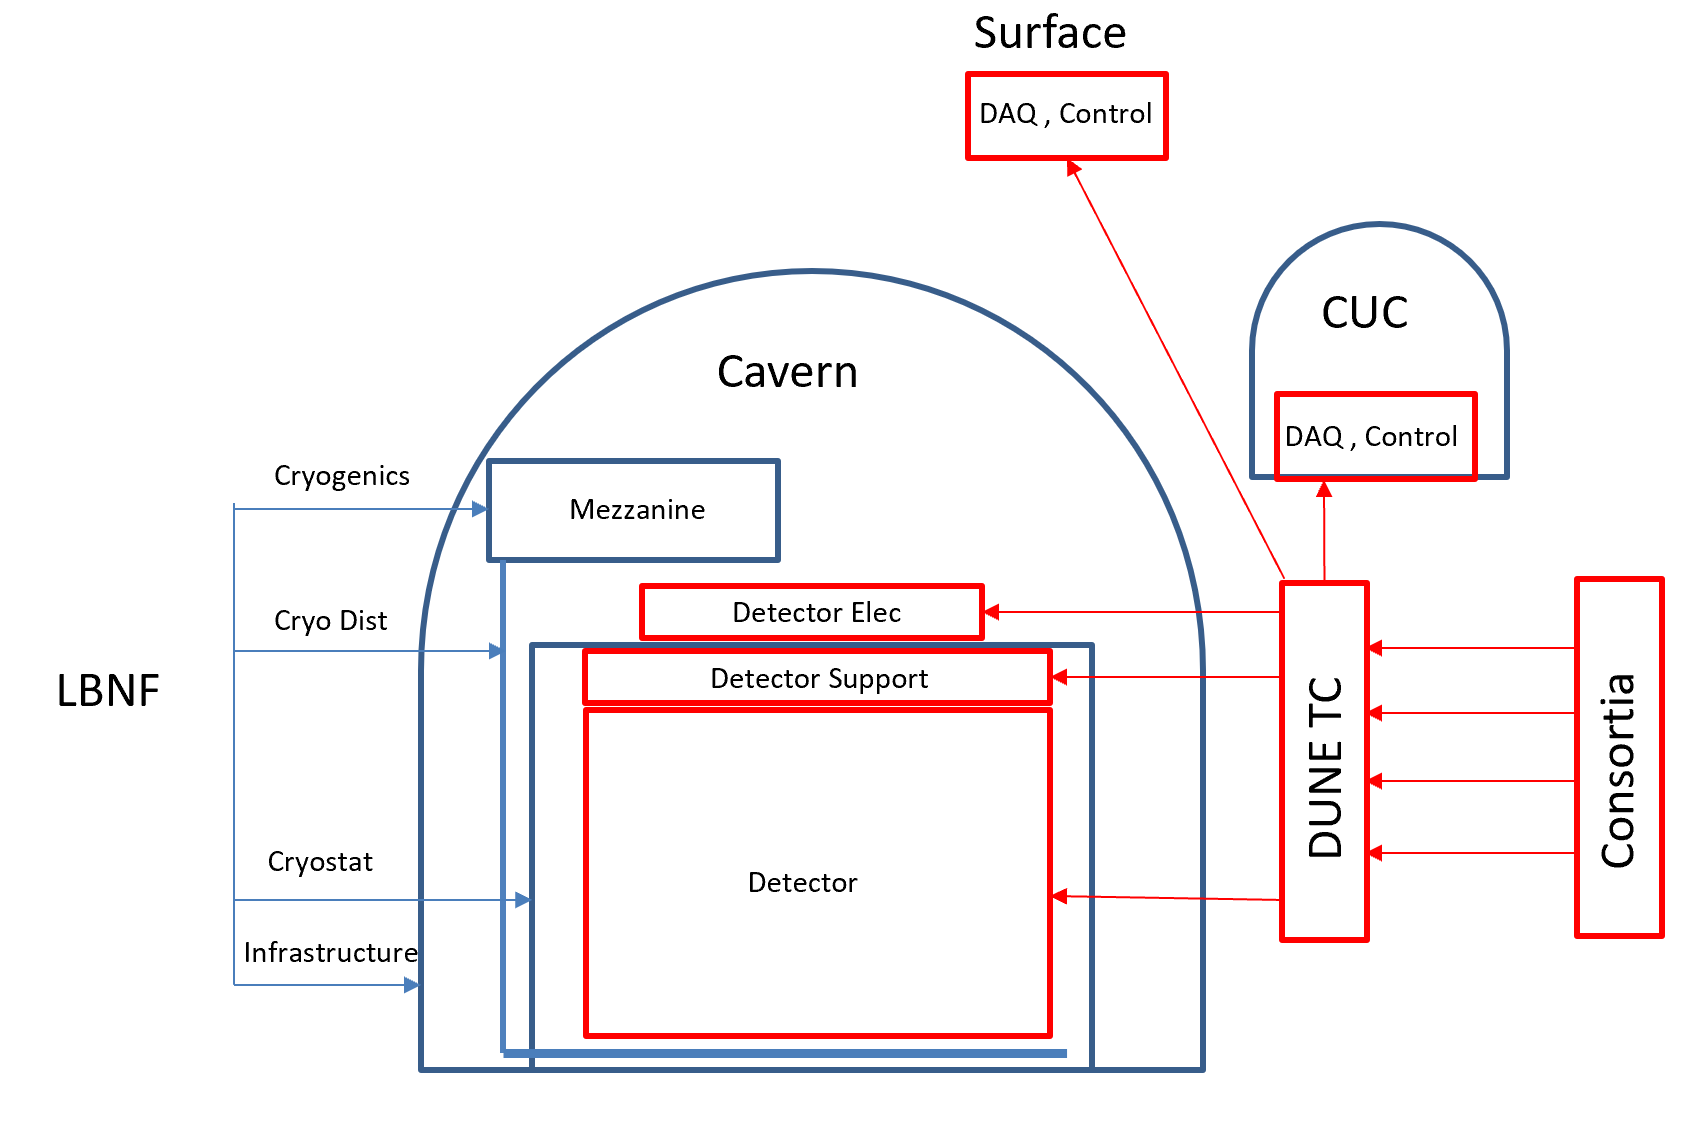
\includegraphics[width=0.7\textwidth]{Integration_nodes.png}
\end{dunefigure}
Figure~\ref{fig:integration_nodes} shows the interfaces between the
detector and facilities. In this figure, within the cavern, items
provided by \dword{lbnf} are on the left and the items provided by
\dword{dune} are on the right. In addition, the \dword{jpo}/\dword{tc} engineering
team integrates (insures that the interfaces are appropriately defined
and managed) the \dword{daq} room in the \dword{cuc} and surface
control and network rooms. Interfaces with \dword{lbnf}
are managed at the boundaries of each integration node. As an example,
the interface between \dword{lbnf} and \dword{dune} for the
underground \dword{daq} and control rooms are power, cooling water,
data fibers and cable penetrations at the room
boundaries. \dword{dune} is responsible for implementing power,
cooling water, data, and signal cables, as well as integrating the
racks.


Interface documents are developed and maintained to manage the
interfaces between consortia and between each consortium and the
\dword{tcoord}. A single document covers the interface between any two
systems, so any one system may have several interface documents. If no
interface exists the interface document is not provided.  The
interface documents are managed by the appropriate consortium
technical leads and by \dword{tc} project engineers.

The content of interface documents varies depending on the type
of interface. However, the documents are intended to have
a common structure: 
\begin{comment}  Too wordy, copied below. Anne
\begin{enumerate}
 \item Definition: This section defines the interfacing systems.
 \item Hardware: In this section, the interfacing hardware components,
   electrical and mechanical, are defined in general terms. As an
   example, the \dword{apa} frame needs to support the \dword{pd}
   mounting brackets.
 \item Design: In this section, the dependencies in design
   methodology, sequence, and standards are described. As with the
   previous example, the design of the \dword{pd} mounting
   brackets depends on side tubes chosen for the \dword{apa}.
 \item Production: Component production and overall assembly is
   shared among interfacing systems. This section details who has what
   responsibilities.
 \item Testing: Like production, testing is a shared
   responsibility. In this section, responsibilities for testing and
   the required equipment are apportioned.
 \item Integration: The integration of systems into installable units
   before insertion into the cryostat is defined in this section. The
   location, methodology, tooling, and environment for integration are
   defined.
 \item Installation: Installation tasks and responsibilities, once
   installable units are assembled, are defined in this section. Any
   special transportation or installation tool or fixture is also
   defined.
 \item Commissioning: In this section, overall responsibilities for
   commissioning tasks are defined, and parameters are set.
 \item Data format, control and error codes: Communications protocols,
   responses and necessary actions are defined.
 \item Appendices: Technical figures and interfaces should be included
   in this section in as much detail as necessary. Block diagrams that
   show interconnections and detailed documentation of each connection
   are needed.
\end{enumerate}
\end{comment}
\begin{enumerate}
 \item Definition: defines the interfacing systems.
 \item Hardware: defines the interfacing hardware components,
   electrical and mechanical, in general terms. As an
   example, the \dword{apa} frame needs to support the \dword{pd}
   mounting brackets.
 \item Design: describes the dependencies in design
   methodology, sequence, and standards. As with the
   previous example, the design of the \dword{pd} mounting
   brackets depends on the side tubes chosen for the \dword{apa}.
 \item Production: details responsibilities for component production
   and overall assembly, which may be shared among interfacing
   systems.
 \item Testing: details responsibilities for testing the required
   equipment. Like production, testing is a shared responsibility.
 \item Integration: defines the integration of systems into installable units
   before insertion into the cryostat. 
   Also defines the location, methodology, tooling, and environment for integration.
 \item Installation: defines installation tasks and responsibilities, once
   installable units are assembled, and  defines  
   special transportation or installation tools or fixtures. 
 \item Commissioning: defines overall responsibilities for
   commissioning tasks  and sets parameters. 
 \item Data format, control and error codes: Communications protocols,
   responses and necessary actions are defined.
 \item Appendices: includes technical figures and interfaces 
   in as much detail as necessary. Must include block diagrams that
   show interconnections and detailed documentation of each connection.
\end{enumerate}


The interface documents will be developed and modified during the
technical design period. At the time of this writing, not all
documents have been fully developed. Once the technical design is
finished, the interface documents will be placed under revision
control. A summary of the interface documents is provided in
Section~\ref{sec:fdsp-coord-interface}.

\section{Engineering Change Control}
\label{sec:fdsp-change}

Changes in design and fabrication requirements follow revision
processes for design and fabrication documents, per individual
consortium practice, while ensuring appropriate levels of
verification, review and approval by the consortium design authority.

Either a consortium or \dword{jpo}/\dword{tc} may initiate and request
changes in design and fabrication requirements that involve interfaces
among consortia and between consortia and \dword{jpo}/\dword{tc}.  The
\dword{jpo}/\dword{tc} team handles such changes through the
\dword{tb}. Any change that affects cost or schedule must be approved
by the \dword{eb}.

When shop or site work must be performed before a given 
design
document under configuration management can be formally revised and re-issued, 
an \dword{ecr} must be developed, approved and distributed. 
Inter-discipline reviews shall be
performed when the \dword{ecr} subject matter may impact other
subsystems. The design authority shall indicate if it is a one-time
change or if the change shall be incorporated into the design
documents. 



\section{Value Engineering}
\label{sec:fdsp-coord-ve}

Value engineering is the process of arriving at cost-effective
solutions to the technical challenges of building the \dword{dune}
detector. \dword{dune} value engineering builds on significant
developments in \dword{lar} detectors dating to the early 1970s,
especially the large \dwords{lartpc}: \dword{icarus} and
\dword{microboone}. Prototyping by both \dword{lbne} and \dword{lbno} has
significantly advanced the value engineering process, leading to
construction of the \dword{protodune} detectors. These detectors validate
\dword{dune} designs and confirm that the necessary performance is
met. Any significant departure from current designs must account for
the success of \dword{protodune}  and may require testing in a second
run of \dword{protodune} to validate that the change does not degrade performance. 

The value engineering process is executed at both the consortium and
\dword{jpo}/\dword{tc} level. For example, the \dword{apa} size has been optimized
over the last 10--15 years, using input from dimensions of the Ross
Shaft, shipping container size, and availability of high-quality long
stainless steel tubes from reliable vendors.  At this point, any
significant change to the \dword{apa} design would likely lead to new
and significant re-engineering costs.

Value engineering is ongoing at all stages of design and will continue
through the fabrication, assembly and installation phases. In
particular, during the fabrication and assembly stages, when labor costs
are relatively higher, it can result in significant cost savings. The
consortia and \dword{jpo}/\dword{tc} are actively engaged and have the necessary
experience for this ongoing process.
